%=======================================================================
\chapter{\tuprolog{} Libraries}
\label{ch:standard-libraries}
%=======================================================================

Libraries are the means by which \tuprolog{} achieves its
fundamental characteristics of minimality and configurability.
%
The engine is by design choice a minimal, purely-inferential core, which includes only the small set of \emph{built-in}s introduced in the previous Chapter.
%
Any other piece of functionality, in the form of predicates, functors, flags and operators, is delivered by \textit{libraries}, which can be loaded and unloaded to/from the engine at any time: each library can provide a set of predicates, functors and a related theory, which can be used to define new flags and operators.

The dynamic loading of libraries can be exploited, for instance, to bound the availability of some functionalities to a specific use context, as in the following example:
%
\begin{verbatim}
% println/1 is defined in ExampleLibrary
run_test(Test, Result) :- run(Test, Result),
                          load_library('ExampleLibrary'),
                          println(Result),
                          unload_library(ExampleLibrary').
\end{verbatim}
%
%The library name can be different from its fully qualified class name.

\noindent The \tuprolog{} distribution include several standard libraries, some of which are loaded by default into any engine--although it is always possible both to create an engine with no pre-loaded libraries, and to create an engine with different (possibly user-defined or third party) pre-loaded libraries.

The fundamental libraries, loaded by default, are the following:
%
\begin{description}

\item[BasicLibrary] (class \texttt{alice.tuprolog.lib.BasicLibrary}) |
    provides the most common Prolog predicates, functors, and operators.
    In order to separate computation and interaction aspects, no I/O
    predicates are included.

\item[ISOLibrary] (class \texttt{alice.tuprolog.lib.ISOLibrary}) |
    provides predicates and functors that are part of the built-in
    section in the ISO standard \cite{iso95}, and are not provided as
    built-ins or by BasicLibrary.

\item[IOLibrary] (class \texttt{alice.tuprolog.lib.IOLibrary}) |
    provides the classic Prolog I/O predicates, except for the ISO-I/O ones.

\item[JavaLibrary] (class \texttt{alice.tuprolog.lib.JavaLibrary}) |
    provides predicates and functors to support multi-paradigm programming
    between Prolog and Java, enabling a complete yet easy access to the
    object-oriented world of Java from \tuprolog{}: features include the
    creation and access of both existing and new objects, classes,
    and resources.
    In the .NET version of \tuprolog{}, this library is replaced\footnote{%
    Actually, integrated: please see Chapter \ref{ch:mpp-in-dotnet} for details.} by \textbf{OOLibrary}, which extends the multi-paradigm programming approach to virtually any language supported by the .NET platform (Chapter \ref{ch:mpp-in-dotnet}.)

\item[ThreadLibrary] (class \texttt{alice.tuprolog.lib.ThreadLibrary}) |
    provides primitives for explicit multi-thread handling  (new in \tuprolog{} 2.7).

\end{description}

\noindent Other libraries included in the standard \tuprolog{} distribution, but not loaded by default, are the following:

\begin{description}

\item[DCGLibrary] (class \texttt{alice.tuprolog.lib.DCGLibrary}) |
    provides support for Definite Clause Grammar, an extension of context
    free grammars used for describing natural and formal languages.

\item[ISOIOLibrary] (class \texttt{alice.tuprolog.lib.ISOIOLibrary}) |
    extends the above IOLibrary by adding ISO-compliant I/O predicates
    (new in \tuprolog{} 2.6).

\item[SocketLibrary] (class \texttt{alice.tuprolog.lib.SocketLibrary}) |
    provides support for TCP and UDP sockets (new in \tuprolog{} 2.7).
\end{description}

\noindent Further libraries exist that are \textit{not} included in the standard \tuprolog{} distribution, because of their very specific domain: they can be downloaded from the \tuprolog{} site, along with their documentation.
%
Among these, for instance, \texttt{RDFLibrary} (class \texttt{alice.tuprolog.lib.RDFLibrary}) provides predicates and functors to handle RDF documents, etc.

The next Sections present the predicates, functors, operators and flag of each library, as well as the dependencies from other libraries, \textit{except for JavaLibrary}, which is discussed in detail in the context of multi-paradigm programming (Chapter \ref{ch:mpp-in-java}, or Chapter \ref{ch:mpp-in-dotnet} for its counterpart in .NET).
%
Throughout this chapter, \texttt{string} means a single-quoted or double-quoted string, as detailed in Chapter \ref{ch:engine}, while \texttt{expr} means an evaluable expression---that is, a term that can be interpreted as a value by some library functors.

%-----------------------------------------------------------------------
\section{BasicLibrary}
\label{sec:basic-library}
%-----------------------------------------------------------------------

%---------------------------------------------------------------------
\subsection{Predicates}
%---------------------------------------------------------------------

%---------------------------------------------------------------------
\subsubsection{Type Testing}
%---------------------------------------------------------------------

\begin{itemize}
 \item \bti{constant/1}\\
    \noindent\bt{constant(X)} is true iff \bt{X} is a constant value.

    \template{constant(@term)}

 \item \bti{number/1}\\
    \noindent\bt{number(X)} is true iff \bt{X} is an integer or a float.

    \template{number(@term)}

 \item \bti{integer/1}\\
    \noindent\bt{integer(X)} is true iff \bt{X} is an integer.

    \template{integer(@term)}

 \item \bti{float/1}\\
    \noindent\bt{float(X)} is true iff \bt{X} is an float.

    \template{float(@term)}

 \item \bti{atom/1}\\
    \noindent\bt{atom(X)} is true iff \bt{X} is an atom.

    \template{atom(@term)}

 \item \bti{compound/1}\\
    \noindent\bt{compound(X)} is true iff \bt{X} is a compound term, that is neither atomic nor a variable.

    \template{compound(@term)}

 \item \bti{var/1}\\
    \noindent\bt{var(X)} is true iff \bt{X} is a variable.

    \template{var(@term)}

 \item \bti{nonvar/1}\\
    \noindent\bt{nonvar(X)} is true iff \bt{X} is not a variable.

    \template{nonvar(@term)}

 \item \bti{atomic/1}\\
    \noindent\bt{atomic(X)} is true iff \bt{X} is atomic (that is is an atom, an integer or a float).

    \template{atomic(@term)}

 \item \bti{ground/1}\\
    \noindent\bt{ground(X)} is true iff \bt{X} is a ground term.

    \template{ground(@term)}

 \item \bti{list/1}\\
    \noindent\bt{list(X)} is true iff \bt{X} is a list.

    \template{list(@term)}
\end{itemize}

%---------------------------------------------------------------------
\subsubsection{Term Creation, Decomposition and Unification}
%---------------------------------------------------------------------

\begin{itemize}

\item \verb|'=..'/2| : \textit{univ}\\
    \noindent\verb|'=..'(Term, List)| is true if \bt{List} is a list consisting of the functor and all arguments of \bt{Term}, in this order.

    \template{'=..'(?term, ?list)}

\item \bti{functor/3}\\
    \noindent\bt{functor(Term, Functor, Arity)} is true if the term \bt{Term} is a compound term, \bt{Functor} is its functor, and \bt{Arity} (an integer) is its arity; or if \bt{Term} is an atom or number equal to \bt{Functor} and \bt{Arity} is 0.

    \template{functor(?term, ?term, ?integer)}

\item \bti{arg/3}\\
    \noindent\bt{arg(N, Term, Arg)} is true if \bt{Arg} is the \bt{N}th
    arguments of \bt{Term} (counting from 1).

    \template{arg(@integer, @compound, -term)}

    \exception{error(instantiation\_error, instantiation\_error(\\
    Goal, ArgNo))} if \texttt{N} or \texttt{Term} are variables. \texttt{Goal} is the goal where the problem occurred, \texttt{ArgNo} indicates the argument that caused the problem (here, \texttt{1} or \texttt{2}).

    \exception{error(type\_error(ValidType, Culprit), type\_error(\\
    Goal, ArgNo, ValidType, Culprit))} if \texttt{N} is not an integer number or \texttt{Term} is not a compound term. \texttt{Goal} is the goal where the problem occurred, \texttt{ArgNo} indicates the argument that caused the problem (here, \texttt{1} or \texttt{2}), \texttt{ValidType} is the expected data type (\texttt{integer} or \texttt{compound}, respectively), \texttt{Culprit} is the wrong term found (either \texttt{N} or \texttt{Term}).

    \exception{error(domain\_error(ValidDomain, Culprit), domain\_\\
    error(Goal, ArgNo, ValidDomain, Culprit))} if \texttt{N} is an int value less than 1. \texttt{Goal} is the goal where the problem occurred, \texttt{ArgNo} indicates the argument that caused the problem (clearly, \texttt{1}), \texttt{ValidDomain} is the expected domain (\texttt{greater\_than\_zero}, respectively), \texttt{Culprit} is the wrong term found (obviously, \texttt{N}).

\item \bti{text\_term/2}\\
    \noindent\bt{text\_term(Text, Term)} is true iff \bt{Text} is the text representation of the term \bt{Term}.

    \template{text\_term(?text, ?term)}

\item \bti{text\_concat/3}\\
    \noindent\bt{text\_concat(Text1, Text2, TextDest)} is
    true iff \bt{TextDest} is the text resulting by appending the text
    \bt{Text2} to \bt{Text1}.

    \template{text\_concat(@string, @string, -string)}

    \exception{error(instantiation\_error, instantiation\_error(\\
    Goal, ArgNo))} if \texttt{Text1} or \texttt{Text2} are variables. \texttt{Goal} is the goal where the problem occurred, \texttt{ArgNo} indicates the argument that caused the problem (here, \texttt{1} or \texttt{2}).

    \exception{error(type\_error(ValidType, Culprit), type\_error(\\
    Goal, ArgNo, ValidType, Culprit))} if \texttt{Text1} or \texttt{Text2} are not atoms. \texttt{Goal} is the goal where the problem occurred, \texttt{ArgNo} indicates the argument that caused the problem (here, \texttt{1} or \texttt{2}),
    \texttt{ValidType} is the expected data type (e.g. \texttt{atom}), \texttt{Culprit} is the wrong term found (either \texttt{Text1} or \texttt{Text2}).

\item \bti{num\_atom/2}\\
    \noindent\bt{num\_atom(Number, Atom)} succeeds iff \bt{Atom} is the atom representation of the number \bt{Number}

    \template{number\_codes(+number, ?atom)}

    \template{number\_codes(?number, +atom)}

    \exception{error(type\_error(ValidType, Culprit), type\_error(\\
    Goal, ArgNo, ValidType, Culprit))} if \texttt{Atom} is a variable and \texttt{Number} is not a number, or, viceversa, if \texttt{Atom} is not an atom. \texttt{Goal} is the goal where the problem occurred, \texttt{ArgNo} indicates the argument that caused the problem (here, \texttt{1} or \texttt{2}), \texttt{ValidType} is the expected data type for the wrong argument (e.g. either \texttt{number} or \texttt{atom}), \texttt{Culprit} is the wrong term found (either \texttt{Number} or \texttt{Atom}).

    \exception{error(domain\_error(ValidType, Culprit), domain\_\\
    error(Goal, ArgNo, ValidDomain, Culprit))} if \texttt{Atom} is an atom that does not represent a number. \texttt{Goal} is the goal where the problem occurred, \texttt{ArgNo} indicates the argument that caused the problem (clearly, \texttt{2}), \texttt{ValidDomain} is the expected domain for the wrong argument (\texttt{num\_atom}), \texttt{Culprit} is the wrong term found (obviously \texttt{Atom}).

\end{itemize}

%---------------------------------------------------------------------
\subsubsection{Occurs Check}
%---------------------------------------------------------------------

\noindent When the process of unification takes place between a variable $S$ and a term $T$, the first thing a Prolog engine should do before proceeding is to check that $T$ does not contain any occurrences of $S$.
This test is known as \emph{occurs check} \cite{ss94} and is conceptually necessary to prevent the unification of terms such as $s(X)$ and $X$, for which no finite common instance exists; yet, the test implies a performance drawback that impacts on the speed and efficiency of the resolution process.

For this reason, most Prolog implementations omit the occur check from their unification algorithm, providing a specific predicate for ``augmented unification'' (that is, unification including the occurs check), to be used when the programmer wants to stay on the safer side:

\begin{itemize}
\item \bti{unify\_with\_occurs\_check/2}\\
    \noindent\bt{unify\_with\_occurs\_check(X, Y)} is true iff \bt{X} and \bt{Y} are unifiable.

    \template{unify\_with\_occurs\_check(?term, ?term)}

\end{itemize}

\noindent \tuprolog{} is an exception in this panorama, because its unification algorithm \textit{always performs the occurs check}: the \bti{unify\_with\_occurs\_check/2} is supported, but is merely a renaming of the standard \texttt{=/2} unification operator.

As a consequence, goals like \texttt{X=f(X)}, that may loop or be solved in an ``infinite'' form in other Prolog systems\footnote{SICStus Prolog, for instance, succeeds returning a solution like \texttt{X=f(f(f(f(f(f(f(f(f(f(...))))))))))}, where the inner dots ``hide'' the infinite self-substitution.}, are occurs-checked in \tuprolog, leading to a failure.


%---------------------------------------------------------------------
\subsubsection{Expression and Term Comparison}
%---------------------------------------------------------------------
\begin{itemize}
    \item expression comparison (generic template:
    \emph{pred}(@expr, @expr)):\\
        \verb|'=:=', '=\=', '>', '<', '>=', '=<'|;

    \item term comparison (generic template:
    \emph{pred}(@term, @term)):\\
         \verb|'==', '\==', '@>', '@<', '@>=', '@=<'|.
\end{itemize}

%---------------------------------------------------------------------
\subsubsection{Finding Solutions}
%---------------------------------------------------------------------
\begin{itemize}
%
\item \bti{findall/3}\\
    \noindent\bt{findall(Template, Goal, List)} is true if and only if
    \bt{List} unifies with the list of values to which a variable X not
    occurring in \bt{Template} or \bt{Goal} would be instantiated
    by successive re-executions of \bt{call(Goal), X = Template} after systematic replacement of all variables in X by new variables.

    \template{\bt{findall(?term, +callable\_term, ?list)}}

    \exception{error(instantiation\_error, instantiation\_error(\\
    Goal, ArgNo))} if \texttt{G} is a variable. \texttt{Goal} is the goal where the problem occurred, \texttt{ArgNo} indicates the argument that caused the problem (obviously, \texttt{1}).

    \exception{error(type\_error(ValidType, Culprit), type\_error(\\
    Goal, ArgNo, ValidType, Culprit))} if \texttt{G} is not a callable goal (for instance, it is a number). \texttt{Goal} is the goal where the problem occurred, \texttt{ArgNo} indicates the argument that caused the problem (here, \texttt{2}), \texttt{ValidType} is the expected data type (\texttt{callable}), \texttt{Culprit} is the wrong term found.

\item \bti{bagof/3}\\
    \noindent\bt{bagof(Template, Goal, Instances)} is true if \bt{Instances} is a non-empty list of all terms such that each unifies with \bt{Template} for a fixed instance W of the variables of \bt{Goal} that are free with respect to \bt{Template}. The ordering of the elements of \bt{Instances} is the order in which the solutions are found.

    \template{bagof(?term, +callable\_term, ?list)}

    \exception{error(instantiation\_error, instantiation\_error(\\
    Goal, ArgNo))} if \texttt{G} is a variable. \texttt{Goal} is the goal where the problem occurred, \texttt{ArgNo} indicates the argument that caused the problem (obviously, \texttt{1}).

    \exception{error(type\_error(ValidType, Culprit), type\_error(\\
    Goal, ArgNo, ValidType, Culprit))} if \texttt{G} is not a callable goal (for instance, it is a number). \texttt{Goal} is the goal where the problem occurred, \texttt{ArgNo} indicates the argument that caused the problem (here, \texttt{2}), \texttt{ValidType} is the expected data type (\texttt{callable}), \texttt{Culprit} is the wrong term found.

\item \bti{setof/3}\\
    \noindent\bt{setof(Template, Goal, List)} is true if \bt{List} is a sorted non-empty list of all terms that each unifies with \bt{Template} for a fixed instance W of the variables of \bt{Goal} that are free with respect to \bt{Template}.

    \template{\bt{setof(?term, +callable\_term, ?list)}}

    \exception{error(instantiation\_error, instantiation\_error(\\
    Goal, ArgNo))} if \texttt{G} is a variable. \texttt{Goal} is the goal where the problem occurred, \texttt{ArgNo} indicates the argument that caused the problem (obviously, \texttt{1}).

    \exception{error(type\_error(ValidType, Culprit), type\_error(\\
    Goal, ArgNo, ValidType, Culprit))} if \texttt{G} is not a callable goal (for instance, it is a number). \texttt{Goal} is the goal where the problem occurred, \texttt{ArgNo} indicates the argument that caused the problem (here, \texttt{2}), \texttt{ValidType} is the expected data type (\texttt{callable}), \texttt{Culprit} is the wrong term found.

\end{itemize}

%---------------------------------------------------------------------
\subsubsection{Control Management}
%---------------------------------------------------------------------
\begin{itemize}
%
\item \bti{(->)/2} : \textit{if-then}\\
\noindent\verb|'->'(If, Then)| is true if and only if \bt{If} is true
and \bt{Then} is true for the first solution of \bt{If}.
%
\item \bti{(;)/2} : \textit{if-then-else}\\
\noindent\verb|';'(Either, Or)| is true iff either \bt{Either} or
\bt{Or} is true.

\item \bti{call/1}\\
    \noindent\bt{call(Goal)} is true if and only if \bt{Goal}
    represents a goal which is true. It is opaque to cut.

    \template{call(+callable\_term)}

    \exception{} the same as the built-in predicate \verb|$call/1|; the exception results to be raised by the auxiliary predicate \texttt{call\_guard(G)}.

\item \bti{once/1}\\
    \noindent\bt{once(Goal)} finds exactly one solution to \bt{Goal}. It is equivalent to \bt{call((Goal, !))} and is opaque to cuts.

    \template{once(@goal)}

\item \bti{repeat/0}\\
    Whenever backtracking reaches \noindent\bt{repeat}, execution proceeds forward again through the same clauses as if another alternative has been found.

    \template{repeat}

\item \verb|'\+'/1| : \textit{not provable}\\
    \noindent\verb|'\+'(Goal)| is the negation predicate and is opaque to cuts. That is, \verb|'\+'(Goal)| is like \bt{call(Goal)} except that its success or failure is the opposite.

    \template{'$\setminus$+'(@goal)}

\item \bti{not/1}\\
    \noindent The predicate \bt{not/1} has the same semantics and implementation as the predicate \verb|'\+'/1|.

    \template{not(@goal)}
\end{itemize}

%---------------------------------------------------------------------
\subsubsection{Clause Retrieval, Creation and Destruction}
%---------------------------------------------------------------------

\noindent Every Prolog engine lets programmers modify its logic
database during execution by adding or deleting specific clauses. The
ISO standard \cite{iso95} distinguishes between static and dynamic
predicates: only the latter can be modified by asserting or retracting
clauses. While typically the \emph{dynamic/1} directive is used to
indicate whenever a user-defined predicate is dynamically modifiable,
\tuprolog{} engines work differently, establishing two default
behaviors: library predicates are always of a static kind; every other
user-defined predicate is dynamic and modifiable at runtime.
%
The following list contains library predicates used to manipulate the
knowledge base of a \tuprolog{} engine during execution.

\begin{itemize}

\item \bti{clause/2}\\
    \noindent\bt{clause(Head, Body)} is true iff \bt{Head} matches the head of a dynamic predicate, and \bt{Body} matches its body. The body of a fact is considered to be \bt{true}. \bt{Head} must be at least partly instantiated.

    \template{\bt{clause(@term, -term)}}

    \exception{error(instantiation\_error, instantiation\_error(\\
    Goal, ArgNo))} if \texttt{Head} is a variable. \texttt{Goal} is the goal where the problem occurred, \texttt{ArgNo} indicates the argument that caused the problem (obviously, \texttt{1}).

\item \bti{assert/1}\\
    \noindent\bt{assert(Clause)} is true and adds \bt{Clause} to the end of the database.

    \template{\bt{assert(@term)}}

    \exception{} the same as the built-in predicate \texttt{assertz/1}.

\item \bti{retract/1}\\
    \noindent\bt{retract(Clause)} removes from the knowledge base a dynamic clause that matches \texttt{Clause} (which must be at least partially instantiated). Multiple solutions are given upon backtracking.

    \template{\bt{retract(@term)}}

    \exception{} the same as the built-in predicate \verb|$retract/1|; the exception is raised by the auxiliary predicate \texttt{retract\_guard(Clause)}.

\item \bti{retractall/1}\\
    \noindent\bt{retractall(Clause)} removes from the knowledge base all the dynamic clauses matching with \texttt{Clause} (which must be at least partially instantiated).

    \template{\bt{retractall(@term)}}

    \exception{} the same as the built-in predicate \verb|$retract/1|; the exception is raised by the auxiliary predicate \texttt{retract\_guard(Clause)}.

\end{itemize}

%---------------------------------------------------------------------
\subsubsection{Operator Management}
%---------------------------------------------------------------------
\begin{itemize}

\item \bti{current\_op/3}\\
    \noindent\bt{current\_op(Priority, Type, Name)} is true iff \bt{Priority} is an integer in the range [0, 1200], \bt{Type} is one of the \bt{fx}, \bt{xfy}, \bt{yfx}, \bt{xfx} values and \bt{Name} is an atom, and as side effect it adds a new operator to the engine operator list.

    \template{current\_op(?integer, ?term, ?atom)}
\end{itemize}

%---------------------------------------------------------------------
\subsubsection{Flag Management}
%---------------------------------------------------------------------
\begin{itemize}
\item \bti{current\_prolog\_flag/2}\\
    \noindent\bt{current\_prolog\_flag(Flag,Value)} is true if the value of the flag \bt{Flag} is \bt{Value}

    \template{current\_prolog\_flag(?atom,?term)}

\item \bti{flag\_list/1}\\
    \noindent\bt{flag\_list(FlagList)} unifies \bt{FlagList} with the list of currently active flags.

    \template{flag\_list(?term)}
\end{itemize}

%---------------------------------------------------------------------
\subsubsection{Actions on Theories and Engines}
%---------------------------------------------------------------------
\begin{itemize}

\item \bti{set\_theory/1}\\
    \noindent\bt{set\_theory(TheoryText)} is true iff \bt{TheoryText}
    is the text representation of a valid \tuprolog{} theory, with the
    side effect of setting it as the new theory of the engine.

    \template{set\_theory(@string)}

    \exception{error(instantiation\_error, instantiation\_error(\\
    Goal, ArgNo))} if \texttt{TheoryText} is a variable. \texttt{Goal} is the goal where the problem occurred, \texttt{ArgNo} indicates the argument that caused the problem (obviously, \texttt{1}).

    \exception{error(type\_error(ValidType, Culprit), type\_error(\\
    Goal, ArgNo, ValidType, Culprit))} if \texttt{TheoryText} is not an atom (i.e. a string). \texttt{Goal} is the goal where the problem occurred, \texttt{ArgNo} indicates the argument that caused the problem (here, \texttt{1}), \texttt{ValidType} is the expected data type (\texttt{atom}), \texttt{Culprit} is the wrong term found.

    \exception{error(syntax\_error(Message), syntax\_error(Goal,\\Line, Position, Message))} if \texttt{TheoryText} is not a valid theory. \texttt{Goal} is the goal where the problem occurred, \texttt{Message} describes the error occurred, \texttt{Line} and \texttt{Position} report the error line and position inside the theory, respectively; if the engine is unable to provide either of them, the corresponding value is set to \texttt{-1}.

\item \bti{add\_theory/1}\\
    \noindent\bt{add\_theory(TheoryText)} is true iff \bt{TheoryText}
    is the text representation of a valid \tuprolog{} theory, with the
    side effect of appending it to the current theory of the engine.

    \template{add\_theory(@string)}

    \exception{error(instantiation\_error, instantiation\_error(\\Goal, ArgNo))} if \texttt{TheoryText} is a variable. \texttt{Goal} is the goal where the problem occurred, \texttt{ArgNo} indicates the argument that caused the problem (obviously, \texttt{1}).

    \exception{error(type\_error(ValidType, Culprit), type\_error(\\
    Goal, ArgNo, ValidType, Culprit))} if \texttt{TheoryText} is not an atom (i.e. a string). \texttt{Goal} is the goal where the problem occurred, \texttt{ArgNo} indicates the argument that caused the problem (here, \texttt{1}), \texttt{ValidType} is the expected data type (\texttt{atom}), \texttt{Culprit} is the wrong term found.

    \exception{error(syntax\_error(Message), syntax\_error(Goal,\\Line, Position, Message))} if \texttt{TheoryText} is not a valid theory. \texttt{Goal} is the goal where the problem occurred, \texttt{Message} describes the error occurred, \texttt{Line} and \texttt{Position} report the error line and position inside the theory, respectively; if the engine is unable to provide either of them, the corresponding value is set to \texttt{-1}.

\item \bti{get\_theory/1}\\
    \noindent\bt{get\_theory(TheoryText)} is true, and
    \bt{TheoryText} is the text representation of the current theory of the engine.

    \template{get\_theory(-string)}

\item \bti{agent/1}\\
    \noindent\bt{agent(TheoryText)} is true, and spawns a
    \tuprolog{} agent with the knowledge base provided as a Prolog
    textual form in \texttt{TheoryText} (the goal is described in the
    knowledge base).

    \template{agent(@string)}

    \exception{error(instantiation\_error, instantiation\_error(\\
    Goal, ArgNo))} if \texttt{TheoryText} is a variable. \texttt{Goal} is the goal where the problem occurred, \texttt{ArgNo} indicates the argument that caused the problem (obviously, \texttt{1}).

    \exception{error(type\_error(ValidType, Culprit), type\_error(\\
    Goal, ArgNo, ValidType, Culprit))} if \texttt{TheoryText} is not an atom (i.e. a string). \texttt{Goal} is the goal where the problem occurred, \texttt{ArgNo} indicates the argument that caused the problem (here, \texttt{1}), \texttt{ValidType} is the expected data type (\texttt{atom}), \texttt{Culprit} is the wrong term found.

\item \bti{agent/2}\\
    \noindent\bt{agent(TheoryText, Goal)} is true, and spawn a
    \tuprolog{} agent with the knowledge base provided as a Prolog
    textual form in \texttt{TheoryText}, and solving the query
    \texttt{Goal} as a goal.

    \template{agent(@string, @term)}

    \exception{error(instantiation\_error, instantiation\_error(\\
    Goal, ArgNo))} if either \texttt{TheoryText} or \texttt{G} is a variable. \texttt{Goal} is the goal where the problem occurred, \texttt{ArgNo} indicates the argument that caused the problem (\texttt{1} or \texttt{2}).

    \exception{error(type\_error(ValidType, Culprit), type\_error(\\
    Goal, ArgNo, ValidType, Culprit))} if \texttt{TheoryText} is not an atom (i.e. a string) or \texttt{G} is not a structure. \texttt{Goal} is the goal where the problem occurred, \texttt{ArgNo} indicates the argument that caused the problem (clearly, \texttt{1} or \texttt{2}), \texttt{ValidType} is the expected data type (\texttt{atom} or \texttt{struct}), \texttt{Culprit} is the wrong term found.

\end{itemize}
%
%---------------------------------------------------------------------
\subsubsection{Spy Events}
%---------------------------------------------------------------------
%
During each demonstration, the engine notifies to interested listeners so-called
{\em spy events}, containing informations on its internal state, such as the
current subgoal being evaluated, the configuration of the execution stack and
the available choice points. The different kinds of spy events currently
corresponds to the different states which the virtual machine realizing the
\tuprolog{}'s inferential core can be found into. \textit{Init} events are
spawned whenever the machine initialize a subgoal for execution; \textit{Call}
events are generated when a choice must be made for the next subgoal to be
executed; \textit{Eval} events represent actual subgoal evaluation; finally,
\textit{Back} events are notified when a backtracking occurs during the
demonstration process.
%
\begin{itemize}
\item \bti{spy/0}\\
    \noindent\bt{spy} is true and enables spy event notification.

    \template{spy}

\item \bti{nospy/0}\\
    \noindent\bt{nospy} is true and disables spy event notification.

    \template{nospy}
\end{itemize}

%---------------------------------------------------------------------
\subsubsection{Auxiliary predicates}
%---------------------------------------------------------------------

\noindent The following predicates are provided by the library's theory.

\begin{itemize}

\item \bti{member/2}\\
    \noindent\bt{member(Element, List)} is true iff \bt{Element} is an element of \bt{List}

    \template{member(?term, +list)}

    \exception{error(type\_error(ValidType, Culprit), type\_error(\\
    Goal, ArgNo, ValidType, Culprit))} if \texttt{List} is not a list. \texttt{Goal} is the goal where the problem occurred, \texttt{ArgNo} indicates the argument that caused the problem (clearly, \texttt{2}), \texttt{ValidType} is the expected data type (\texttt{list}), \texttt{Culprit} is the wrong term found.

\item \bti{length/2}\\
    \noindent\bt{length(List, NumberOfElements)} is true in three different cases: (1) if \bt{List} is instantiated to a list of determinate length, then \bt{Length} will be unified with this length; (2) if \bt{List} is of indeterminate length and \bt{Length} is instantiated to an integer, then \bt{List} will be unified with a list of length \bt{Length} and in such a case the list elements are unique variables; (3) if \bt{Length} is unbound then \bt{Length} will be unified with all possible lengths of \bt{List}.

    \template{member(?list, ?integer)}

\item \bti{append/3}\\
    \noindent\bt{append(What, To, Target)} is true iff \bt{Target} list can be obtained by appending the \bt{To} list to the \bt{What} list.

    \template{append(?list, ?list, ?list)}

\item \bti{reverse/2}\\
    \noindent\bt{reverse(List, ReversedList)} is true iff \bti{ReversedList} is the reverse list of \bt{List}.

    \template{reverse(+list, -list)}

    \exception{error(type\_error(ValidType, Culprit), type\_error(\\
    Goal, ArgNo, ValidType, Culprit))} if \texttt{List} is not a list. \texttt{Goal} is the goal where the problem occurred, \texttt{ArgNo} indicates the argument that caused the problem (here, \texttt{1}), \texttt{ValidType} is the expected data type (\texttt{list}), \texttt{Culprit} is the wrong term found.

\item \bti{delete/3}\\
    \noindent\bt{delete(Element, ListSource, ListDest)} is true iff \bt{ListDest} list can be obtained by removing \bt{Element} from the list \bt{ListSource}.

    \template{delete(@term, +list, -list)}

    \exception{error(type\_error(ValidType, Culprit), type\_error(\\
    Goal, ArgNo, ValidType, Culprit))} if \texttt{ListSource} is not a list. \texttt{Goal} is the goal where the problem occurred, \texttt{ArgNo} indicates the argument that caused the problem (here, \texttt{2}), \texttt{ValidType} is the expected data type (\texttt{list}), \texttt{Culprit} is the wrong term found.

\item \bti{element/3}\\
    \noindent\bt{element(Pos, List, Element)} is true iff \bt{Element} is the \bt{Pos}-th element of \bt{List} (element numbering starts from 1).

    \template{element(@integer, +list, -term)}

    \exception{error(type\_error(ValidType, Culprit), type\_error(\\
    Goal, ArgNo, ValidType, Culprit))} if \texttt{List} is not a list. \texttt{Goal} is the goal where the problem occurred, \texttt{ArgNo} indicates the argument that caused the problem (here, \texttt{2}), \texttt{ValidType} is the expected data type (\texttt{list}), \texttt{Culprit} is the wrong term found.

\item \bti{quicksort/3}\\
    \noindent\bt{quicksort(List, ComparisonPredicate, SortedList)} is true iff\\
    \bt{SortedList} contains the same elements as \bt{List}, but sorted according to the criterion defined by \bt{ComparisonPredicate}.

    \template{element(@list, @pred, -list)}
\end{itemize}

%---------------------------------------------------------------------
\subsection{Functors}
%---------------------------------------------------------------------

The following functors for expression evaluation (with the usual semantics) are provided:
\begin{itemize}
    \item unary functors:  \verb|+, -, ~, +|
    \item binary functors:  \verb|+, -, *, \, **, <<, >>, /\, \/|
\end{itemize}

%---------------------------------------------------------------------
\subsection{Operators}
%---------------------------------------------------------------------

The full list of BasicLibrary operators, with their priority and associativity, is reported in Table \ref{tab:basiclibrary-operators}.

Expression comparison operators (\verb|=:=| (equal), \verb|=\=| (different), \verb|>| (greater), \verb|<| (smaller), \verb|>=| (greater or equal), \verb|<=| (smaller or equal)) can raise the following exceptions:

\begin{itemize}

    \item\exception{error(instantiation\_error, instantiation\_error(\\
        Goal, ArgNo))} if any of the arguments is a variable. \texttt{Goal} is the goal where the problem occurred, \texttt{ArgNo} indicates the argument that caused the problem (\texttt{1} or \texttt{2}).

    \item\exception{error(type\_error(ValidType, Culprit), type\_error(\\
        Goal, ArgNo, ValidType, Culprit))} if any of the two arguments is not an evaluable expression. \texttt{Goal} is the goal where the problem occurred, \texttt{ArgNo} indicates the argument that caused the problem (\texttt{1} or \texttt{2}), \texttt{ValidType} is the expected data type (\texttt{evaluable}), \texttt{Culprit} is the wrong term found.

    \item\exception{error(evaluation\_error(Error), evaluation\_error(\\
        Goal, ArgNo, Error))} if an error occurs during the evaluation of any of the two arguments. \texttt{Goal} is the goal where the problem occurred, \texttt{ArgNo} indicates the argument that caused the problem (\texttt{1} or \texttt{2}), \texttt{Error} is the error occurred (e.g. \texttt{zero\_division} in case of a division by zero).

\end{itemize}


\begin{table}[h]
    %
    \begin{center}{\small\tt
    \begin{tabular}{p{2cm}|p{1cm}|p{1cm}}\hline\hline
    Name & Assoc. & Prio. \\ \hline\hline
    :-      &   fx  &   1200 \\
    :-      &   xfx &   1200 \\
    ?-      &   fx  &   1200 \\
    ;       &   xfy &   1100 \\
    ->      &   xfy &   1050 \\
    ,       &   xfy &   1000 \\
    not     &   fy  &   900 \\
    $\setminus$+   &   fy   & 900   \\
    =       &   xfx &   700 \\
    $\setminus$=    &  xfx  &   700 \\
    ==      &   xfx &   700 \\
    $\setminus$==   &  xfx  &   700 \\
    @>      &   xfx & 700   \\
    @<      &   xfx & 700   \\
    @=<    &   xfx & 700   \\
    @>=    &   xfx & 700   \\
    =:=    &   xfx & 700   \\
    =$\setminus$=   &   xfx & 700   \\
    >      &   xfx & 700   \\
    <      &   xfx & 700   \\
    >=      &   xfx & 700   \\
    =<      &   xfx & 700   \\
    is      &   xfx &   700 \\
    =..     &   xfx & 700 \\
    +       &   yfx & 500 \\
    -       &   yfx & 500 \\
    $/\setminus$    &   yfx &   500 \\
    $\setminus/$    &   yfx &   500 \\
    $\ast$  &   yfx & 400 \\
    /       &   yfx & 400 \\
    //      &   yfx & 400 \\
    >>      &   yfx & 400 \\
    <<      &   yfx & 400 \\
    >>      &   yfx & 400 \\
    $\ast$$\ast$  &   xfx & 200 \\
    \textasciicircum  &   xfy & 200 \\
    $\setminus$$\setminus$      &   fx & 200 \\
    -       &   fy & 200 \\
    \hline\hline
    \end{tabular}
    }\end{center}
    \caption{BasicLibrary operators.}\label{tab:basiclibrary-operators}
\end{table}

\clearpage

%-----------------------------------------------------------------------
\section{ISOLibrary}
\label{sec:iso-library}
%-----------------------------------------------------------------------

\noindent \emph{Library Dependencies}: BasicLibrary.

This library contains all the predicates and functors of the Prolog ISO standard and that are not provided directly at the \tuprolog{} core or at the BasicLibrary levels.

%---------------------------------------------------------------------
\subsection{Predicates}
%---------------------------------------------------------------------

%---------------------------------------------------------------------
\subsubsection{Type Testing}
%---------------------------------------------------------------------

\begin{itemize}
\item \bti{bound/1}\\
    \noindent\bt{bound(Term)} is a synonym for the \bt{ground/1} predicate defined in BasicLibrary.

    \template{bound(+term)}

\item \bti{unbound/1}\\
    \noindent\bt{unbound(Term)} is true iff \bt{Term} is not a ground term.

    \template{unbound(+term)}
\end{itemize}

%---------------------------------------------------------------------
\subsubsection{Atoms Processing}
%---------------------------------------------------------------------

\begin{itemize}

\item \bti{atom\_length/2}\\
    \noindent\bt{atom\_length(Atom, Length)} is true iff the integer \bt{Length} equals the number of characters in the name of atom \bt{Atom}.

    \template{atom\_length(+atom, ?integer)}

    \exception{error(instantiation\_error, instantiation\_error(\\
    Goal, ArgNo))} if \texttt{Atom} is a variable. \texttt{Goal} is the goal where the problem occurred, \texttt{ArgNo} indicates the argument that caused the problem (clearly, \texttt{1}).

    \exception{error(type\_error(ValidType, Culprit), type\_error(\\
    Goal, ArgNo, ValidType, Culprit))} if \texttt{Atom} is not an atom. \texttt{Goal} is the goal where the problem occurred, \texttt{ArgNo} indicates the argument that caused the problem (here, \texttt{1}), \texttt{ValidType} is the expected data type (\texttt{atom}), \texttt{Culprit} is the wrong term found.

\item \bti{atom\_concat/3}\\
    \noindent\bt{atom\_concat(Start, End, Whole)} is true iff the \bt{Whole} is the atom obtained by concatenating the characters of \bt{End} to those of \bt{Start}. If \bt{Whole} is instantiated, then all decompositions of \bt{Whole} can be obtained by backtracking.

    \template{atom\_concat(?atom, ?atom, +atom)}

    \template{atom\_concat(+atom, +atom, -atom)}

\item \bti{sub\_atom/5}\\
    \noindent\bt{sub\_atom(Atom, Before, Length, After, SubAtom)} is true iff \bt{Sub}-\bt{Atom} is the sub atom of \bt{Atom} of length \bt{Length} that appears with \bt{Before} characters preceding it and \bt{After} characters following. It is re-executable.

    \template{sub\_atom(+atom, ?integer, ?integer, ?integer, ?atom)}

    \exception{error(type\_error(ValidType, Culprit), type\_error(\\
    Goal, ArgNo, ValidType, Culprit))} if \texttt{Atom} is not an atom. \texttt{Goal} is the goal where the problem occurred, \texttt{ArgNo} indicates the argument that caused the problem (here, \texttt{1}), \texttt{ValidType} is the expected data type (\texttt{atom}), \texttt{Culprit} is the wrong term found.

\item \bti{atom\_chars/2}\\
    \noindent\bt{atom\_chars(Atom,List)} succeeds iff \bt{List} is a list whose elements are the one character atoms that in order make up \bt{Atom}.

    \template{atom\_chars(+atom, ?character\_list)}

    \template{atom\_chars(-atom, ?character\_list)}

    \exception{error(type\_error(ValidType, Culprit), type\_error(\\
    Goal, ArgNo, ValidType, Culprit))} if \texttt{Atom} is a variable and \texttt{List} is not a list, or, conversely, \texttt{List} is a variable and \texttt{Atom} is not an atom. \texttt{Goal} is the goal where the problem occurred, \texttt{ArgNo} indicates the argument that caused the problem (either \texttt{1} or \texttt{2}), \texttt{ValidType} is the expected data type (\texttt{atom} or \texttt{list}, respectively), \texttt{Culprit} is the wrong term found.

\item \bti{atom\_codes/2}\\
    \noindent\bt{atom\_codes(Atom, List)} succeeds iff \bt{List} is a list whose elements are the character codes that in order correspond to the characters that make up \bt{Atom}.

    \template{atom\_codes(+atom, ?character\_code\_list)}

    \template{atom\_chars(-atom, ?character\_code\_list)}

\item \bti{char\_code/2}\\
    \noindent\bt{char\_code(Char, Code)} succeeds iff \bt{Code} is a the character code that corresponds to the character \bt{Char}.

    \template{char\_code(+character, ?character\_code)}

    \template{char\_code(-character, +character\_code)}

    \exception{error(type\_error(ValidType, Culprit), type\_error(\\
    Goal, ArgNo, ValidType, Culprit))} if \texttt{Code} is a variable and \texttt{Char} is not a character (that is, an atom of length 1), or, conversely, \texttt{Char} is a variable and \texttt{Code} is not an integer. \texttt{Goal} is the goal where the problem occurred, \texttt{ArgNo} indicates the argument that caused the problem (either \texttt{1} or \texttt{2}), \texttt{ValidType} is the expected data type (\texttt{character} or \texttt{integer}, respectively), \texttt{Culprit} is the wrong term found.

\item \bti{number\_chars/2}\\
    \noindent\bt{number\_chars(Number, List)} succeeds iff \bt{List} is a list whose elements are the one character atoms that in order make up \bt{Number}.

    \template{number\_chars(+number, ?character\_list)}

    \template{number\_chars(-number, ?character\_list)}

\item \bti{number\_codes/2}\\
    \noindent\bt{number\_codes(Number, List)} succeeds iff \bt{List} is a list whose elements are the codes for the one character atoms that in order make up \bt{Number}.

    \template{number\_codes(+number,?character\_code\_list)}

    \template{number\_codes(-number,?character\_code\_list)}

\end{itemize}

%---------------------------------------------------------------------
\subsection{Functors}
%---------------------------------------------------------------------

\begin{itemize}
    \item Trigonometric functions: \bt{sin(+expr)}, \bt{cos(+expr)}, \bt{atan(+expr)}.
    %
    \item Logarithmic functions: \bt{exp(+expr)}, \bt{log(+expr)}, \bt{sqrt(+expr)}.
    %
    \item Absolute value functions: \bt{abs(+expr)}, \bt{sign(+Expr)}.
    %
    \item Rounding functions: \bt{floor(+expr)},
    \bt{ceiling(+expr)}, \bt{round(+expr)}, \bt{truncate(+expr)},
    \bt{float(+expr)}, \bt{float\_integer\_part(+expr)},\\\bt{float\_fractional\_part(+expr)}.
    %
    \item Integer division functions:
    \bt{div(+expr, +expr)}, \bt{mod(+expr, +expr)}, \bt{rem(+expr, +expr)}.
\end{itemize}

%---------------------------------------------------------------------
\subsection{Operators}
%---------------------------------------------------------------------

The full list of ISOLibrary operators, with their priority and associativity, is reported in Table \ref{tab:isolibrary-operators}.

\begin{table}[h]
    %
    \begin{center}{\small\tt
    \begin{tabular}{p{2cm}|p{1cm}|p{1cm}}\hline\hline
    Name & Assoc. & Prio. \\ \hline
    mod   & yfx & 400\\
    div   & yfx & 300\\
    rem   & yfx & 300\\
    sin   & fx & 200\\
    cos   & fx & 200\\
    sqrt  & fx & 200\\
    atan  & fx & 200\\
    exp   & fx & 200\\
    log   & fx & 200\\
    \hline\hline
    \end{tabular}
    }\end{center}
    \caption{ISOLibrary operators.}\label{tab:isolibrary-operators}
\end{table}

%---------------------------------------------------------------------
\subsection{Flags}
%---------------------------------------------------------------------

The full list of ISOLibrary flags, with their admissible and default values, is reported in Table \ref{tab:isolibrary-flags}.

\begin{table}[h]
    %
    \begin{center}{\small\tt
    \begin{tabular}{p{4.8cm}|p{2.2cm}|p{2.2cm}|p{1.8cm}}\hline\hline
        Flag Name   & Possible Values & Default Value & Modifiable\\ \hline\hline
        bounded          & {true}          &  true        & no\\
        max\_integer     & {2147483647}    &  2147483647  & no\\
        min\_integer     & {-2147483648}   &  -2147483648 & no \\
        integer\_rounding\_function & down & down         & no\\
        char\_conversion & {off}           & off          & no\\
        debug            & {off}           & off          & no\\
        max\_arity       & {2147483647}    & 2147483647   & no\\
        undefined\_predicates & fail       & fail         & no\\
        double\_quotes  &  {atom}          & atom         & no\\
    \hline\hline
    \end{tabular}
    }\end{center}
    \caption{ISOLibrary flags. Any tentative to modify unmodifiable flags will result into a \texttt{permission\_error} exception.}\label{tab:isolibrary-flags}
\end{table}

%-----------------------------------------------------------------------
\section{IOLibrary}
\label{sec:io-library}
%-----------------------------------------------------------------------

\noindent \emph{Library Dependencies}: BasicLibrary.

The IOLibrary defines the classical Prolog I/O predicates; further ISO-compliant I/O predicates are provided by ISOIOLibrary (Section \ref{sec:isoio-library}).

%---------------------------------------------------------------------
\subsection{Predicates}
%---------------------------------------------------------------------

%---------------------------------------------------------------------
\subsubsection{General I/O}
%---------------------------------------------------------------------

\begin{itemize}

\item \bti{see/1}\\
    \noindent\bt{see(StreamName)} is used to create/open an input stream; the predicate is true iff \bt{StreamName} is a string representing the name of a file to be created or accessed as input stream, or the string \texttt{stdin} selecting current standard input as input stream.

    \template{see(@atom)}

    \exception{error(instantiation\_error, instantiation\_error(\\
    Goal, ArgNo))} if \texttt{StreamName} is a variable. \texttt{Goal} is the goal where the problem occurred, \texttt{ArgNo} indicates the argument that caused the problem (obviously, \texttt{1}).

    \exception{error(type\_error(ValidType, Culprit), type\_error(\\
    Goal, ArgNo, ValidType, Culprit))} if \texttt{StreamName} is not an atom. \texttt{Goal} is the goal where the problem occurred, \texttt{ArgNo} indicates the argument that caused the problem (here, \texttt{1}), \texttt{ValidType} is the expected data type (\texttt{atom}), \texttt{Culprit} is the wrong term found.

    \exception{error(domain\_error(ValidDomain, Culprit), domain\_\\
    error(Goal, ArgNo, ValidDomain, Culprit))} if \texttt{StreamName} is not the name of an accessible file. \texttt{Goal} is the goal where the problem occurred, \texttt{ArgNo} indicates the argument that caused the problem (clearly, \texttt{1}), \texttt{ValidDomain} is the expected domain (\texttt{stream}), \texttt{Culprit} is the wrong term found.

\item \bti{seen/0}\\
    \noindent\bt{seen} is used to close the input stream previously opened; the predicate is true iff the closing action is possible

    \template{seen}

\item \bti{seeing/1}\\
    \noindent\bt{seeing(StreamName)} is true iff \texttt{StreamName} is the name of the stream currently used as input stream.

    \template{seeing(?term)}

\item \bti{tell/1}\\
    \noindent\bt{tell(StreamName)} is used to create/open an output stream; the predicate is true iff \bt{StreamName} is a string representing the name of a file to be created or accessed as output stream, or the string \texttt{stdout} selecting current standard output as output stream.

    \template{tell(@atom)}

    \exception{error(instantiation\_error, instantiation\_error(\\
    Goal, ArgNo))} if \texttt{StreamName} is a variable. \texttt{Goal} is the goal where the problem occurred, \texttt{ArgNo} indicates the argument that caused the problem (obviously, \texttt{1}).

    \exception{error(type\_error(ValidType, Culprit), type\_error(\\
    Goal, ArgNo, ValidType, Culprit))} if \texttt{StreamName} is not an atom. \texttt{Goal} is the goal where the problem occurred, \texttt{ArgNo} indicates the argument that caused the problem (here, \texttt{1}), \texttt{ValidType} is the expected data type (\texttt{atom}), \texttt{Culprit} is the wrong term found.

    \exception{error(domain\_error(ValidDomain, Culprit), domain\_\\
    error(Goal, ArgNo, ValidDomain, Culprit))} if \texttt{StreamName} is not the name of an accessible file. \texttt{Goal} is the goal where the problem occurred, \texttt{ArgNo} indicates the argument that caused the problem (clearly, \texttt{1}), \texttt{ValidDomain} is the expected domain (\texttt{stream}), \texttt{Culprit} is the wrong term found.

\item \bti{told/0}\\
    \noindent\bt{told} is used to close the output stream previously opened; the predicate is true iff the closing action is possible.

    \template{told}

\item \bti{telling/1}\\
    \noindent\bt{telling(StreamName)} is true iff \texttt{StreamName} is the name of the stream currently used as input stream.

    \template{telling(?term)}

\item \bti{put/1}\\
    \noindent\bt{put(Char)} puts the character \bt{Char} on current output stream; it is true iff the operation is possible.

    \template{put(@char)}

    \exception{error(instantiation\_error, instantiation\_error(\\
    Goal, ArgNo))} if \texttt{Char} is a variable. \texttt{Goal} is the goal where the problem occurred, \texttt{ArgNo} indicates the argument that caused the problem (obviously, \texttt{1}).

    \exception{error(type\_error(ValidType, Culprit), type\_error(\\
    Goal, ArgNo, ValidType, Culprit))} if \texttt{Char} is not a character, i.e. an atom of length 1. \texttt{Goal} is the goal where the problem occurred, \texttt{ArgNo} indicates the argument that caused the problem (\texttt{1}), \texttt{ValidType} is the expected data type (\texttt{char}), \texttt{Culprit} is the wrong term found.

    \exception{error(permission\_error (Operation, ObjectType,\\
    Culprit), permission\_error(Goal, Operation, ObjectType,\\
    Culprit, Message))} if it was impossible to write on the output stream. \texttt{Goal} is the goal where the problem occurred, \texttt{Operation} is the operation to be performed (here, \texttt{output}), \texttt{ObjectType} is the type of the target object (\texttt{stream}), \texttt{Culprit} is the name of the output stream, and \texttt{Message} provides extra info about the occurred error.

\item \bti{get0/1}\\
    \noindent\bt{get0(Value)} is true iff \bt{Value} is the next character (whose code can span on the entire ASCII codes) available from the input stream, or -1 if no characters are available; as a side effect, the character is removed from the input stream.

    \template{get0(?charOrMinusOne)}

    \exception{error(permission\_error (Operation, ObjectType,\\
    Culprit), permission\_error(Goal, Operation, ObjectType,\\
    Culprit, Message))} if it was impossible to read from the input stream. \texttt{Goal} is the goal where the problem occurred, \texttt{Operation} is the operation to be performed (here, \texttt{input}), \texttt{ObjectType} is the type of the target object (\texttt{stream}), \texttt{Culprit} is the name of the input stream, and \texttt{Message} provides extra info about the occurred error.

\item \bti{get/1}\\
    \noindent\bt{get(Value)} is true iff \bt{Value} is the next character (whose code can span on the range 32..255 as ASCII codes) available from the input stream, or -1 if no characters are available; as a side effect, the character (with all the characters that precede this one not in the range 32..255) is removed from the input stream.

    \template{get(?charOrMinusOne)}

    \exception{error(permission\_error (Operation, ObjectType,\\
    Culprit), permission\_error(Goal, Operation, ObjectType,\\
    Culprit, Message))} if it was impossible to read from the input stream. \texttt{Goal} is the goal where the problem occurred, \texttt{Operation} is the operation to be performed (here, \texttt{input}), \texttt{ObjectType} is the type of the target object (\texttt{stream}), \texttt{Culprit} is the name of the input stream, and \texttt{Message} provides extra info about the occurred error.

\item \bti{tab/1}\\
    \noindent\bt{tab(NumSpaces)} inserts \bt{NumSpaces} space characters (ASCII code 32) on output stream; the predicate is true iff the operation is possible.

    \template{tab(+integer)}

    \exception{error(instantiation\_error, instantiation\_error(\\
    Goal, ArgNo))} if \texttt{NumSpaces} is a variable. \texttt{Goal} is the goal where the problem occurred, \texttt{ArgNo} indicates the argument that caused the problem (obviously, \texttt{1}).

    \exception{error(type\_error(ValidType, Culprit), type\_error(\\
    Goal, ArgNo, ValidType, Culprit))} if \texttt{NumSpaces} is not an integer number. \texttt{Goal} is the goal where the problem occurred, \texttt{ArgNo} indicates the argument that caused the problem (here, \texttt{1}), \texttt{ValidType} is the expected data type (\texttt{integer}), \texttt{Culprit} is the wrong term found.

    \exception{error(permission\_error (Operation, ObjectType,\\
    Culprit), permission\_error(Goal, Operation, ObjectType,\\
    Culprit, Message))} if it was impossible to write on the output stream. \texttt{Goal} is the goal where the problem occurred, \texttt{Operation} is the operation to be performed (here, \texttt{output}), \texttt{ObjectType} is the type of the target object (\texttt{stream}), \texttt{Culprit} is the name of the output stream, and \texttt{Message} provides extra info about the occurred error.

\item \bti{read/1}\\
    \noindent\bt{read(Term)} is true iff \bt{Term} is Prolog term available from the input stream. The term must ends with the \emph{.} character; if no valid terms
    are available, the predicate fails. As a side effect, the term is removed from the input stream.

    \template{read(?term)}

    \exception{error(permission\_error (Operation, ObjectType,\\
    Culprit), permission\_error(Goal, Operation, ObjectType,\\
    Culprit, Message))} if it was impossible to read from the input stream. \texttt{Goal} is the goal where the problem occurred, \texttt{Operation} is the operation to be performed (here, \texttt{input}), \texttt{ObjectType} is the type of the target object (\texttt{stream}), \texttt{Culprit} is the name of the input stream, and \texttt{Message} provides extra info about the occurred error.

    \exception{error(syntax\_error(Message), syntax\_error(Goal,\\
    Line, Position, Message))} if a syntax error occurred when reading from the input stream. \texttt{Goal} is the goal where the problem occurred, \texttt{Message} is the string read from the input that caused the error, while \texttt{Line} and \texttt{Position} are not applicable in this case and therefore default to \texttt{-1}.

\item \bti{write/1}\\
    \noindent\bt{write(Term)} writes the term \bt{Term} on current output stream. The predicate fails if the operation is not possible.

    \template{write(@term)}

    \exception{error(instantiation\_error, instantiation\_error(\\
    Goal, ArgNo))} if \texttt{Term} is a variable. \texttt{Goal} is the goal where the problem occurred, \texttt{ArgNo} indicates the argument that caused the problem (obviously, \texttt{1}).

    \exception{error(permission\_error (Operation, ObjectType,\\
    Culprit), permission\_error(Goal, Operation, ObjectType,\\
    Culprit, Message))} if it was impossible to write on the output stream. \texttt{Goal} is the goal where the problem occurred, \texttt{Operation} is the operation to be performed (here, \texttt{output}), \texttt{ObjectType} is the type of the target object (\texttt{stream}), \texttt{Culprit} is the name of the output stream, and \texttt{Message} provides extra info about the occurred error.

\item \bti{print/1}\\
    \noindent\bt{print(Term)} writes the term \bt{Term} on current output stream, removing apices if the term is an atom representing a string. The predicate fails if the operation is not possible.

    \template{print(@term)}

    \exception{error(instantiation\_error, instantiation\_error(\\
    Goal, ArgNo))} if \texttt{Term} is a variable. \texttt{Goal} is the goal where the problem occurred, \texttt{ArgNo} indicates the argument that caused the problem (obviously, \texttt{1}).

    \exception{error(permission\_error (Operation, ObjectType,\\
    Culprit), permission\_error(Goal, Operation, ObjectType,\\
    Culprit, Message))} if it was impossible to write on the output stream. \texttt{Goal} is the goal where the problem occurred, \texttt{Operation} is the operation to be performed (here, \texttt{output}), \texttt{ObjectType} is the type of the target object (\texttt{stream}), \texttt{Culprit} is the name of the output stream, and \texttt{Message} provides extra info about the occurred error.

\item \bti{nl/0}\\
    \noindent\bt{nl} writes a new line control character on current output stream. The predicate fails if the operation is not possible.

    \template{nl}

    \exception{error(permission\_error (Operation, ObjectType,\\
    Culprit), permission\_error(Goal, Operation, ObjectType,\\
    Culprit, Message))} if it was impossible to write on the output stream. \texttt{Goal} is the goal where the problem occurred, \texttt{Operation} is the operation to be performed (here, \texttt{output}), \texttt{ObjectType} is the type of the target object (\texttt{stream}), \texttt{Culprit} is the name of the output stream, and \texttt{Message} provides extra info about the occurred error.

\end{itemize}

%---------------------------------------------------------------------
\subsubsection{Helper Predicates}
%---------------------------------------------------------------------

\begin{itemize}

\item \bti{text\_from\_file/2}\\
    \noindent\bt{text\_from\_file(File, Text)} is true iff \bt{Text} is the text contained in the file whose name is \texttt{File}.

    \template{text\_from\_file(+string, -string)}

    \exception{error(instantiation\_error, instantiation\_error(\\
    Goal, ArgNo))} if \texttt{File} is a variable. \texttt{Goal} is the goal where the problem occurred, \texttt{ArgNo} indicates the argument that caused the problem (obviously, \texttt{1}).

    \exception{error(type\_error(ValidType, Culprit), type\_error(\\
    Goal, ArgNo, ValidType, Culprit))} if \texttt{File} is not an atom. \texttt{Goal} is the goal where the problem occurred, \texttt{ArgNo} indicates the argument that caused the problem (here, \texttt{1}), \texttt{ValidType} is the expected data type (\texttt{atom}), \texttt{Culprit} is the wrong term found.

    \exception{error(existence\_error(ObjectType, Culprit),\\
    existence\_error(Goal, ArgNo, ObjectType, Culprit, Message))} if \texttt{File} does not exist. \texttt{Goal} is the goal where the problem occurred, \texttt{ArgNo} indicates the argument that caused the problem (clearly, \texttt{1}), \texttt{ObjectType} is the type of the missing object (\texttt{stream}), \texttt{Culprit} is the wrong term found and \texttt{Message} provides an error message (here, most likely \texttt{file\_not\_found}).

\item \bti{agent\_file/1}\\
    \noindent\bt{agent\_file(FileName)} is true iff \texttt{FileName} is an accessible file containing a Prolog knowledge base, and as a side effect it spawns a \tuprolog{} agent provided with that knowledge base.

    \template{agent\_file(+string)}

    \exception{} the predicate maps onto the above \texttt{text\_from\_file(File, Text)} with \texttt{File=FileName}, so the same exceptions are raised.

\item \bti{solve\_file/2}\\
    \noindent\bt{solve\_file(FileName, Goal)} is true iff \texttt{FileName} is an accessible file containing a Prolog knowledge base, and as a side effect it solves the query \texttt{Goal} according to that knowledge base.

    \template{solve\_file(+string, +goal)}

    \exception{} the predicate maps onto the above \texttt{text\_from\_file(File, Text)} with \texttt{File=FileName}, so the same exceptions are raised.

    Moreover, it also raises the following specific exceptions:

    \exception{error(instantiation\_error, instantiation\_error(\\
    Goal, ArgNo))} if \texttt{G} is a variable. \texttt{Goal} is the goal where the problem occurred, \texttt{ArgNo} indicates the argument that caused the problem (in this case, \texttt{2}).

    \exception{error(type\_error(ValidType, Culprit), type\_error(\\
    Goal, ArgNo, ValidType, Culprit))} if \texttt{G} is not a callable goal. \texttt{Goal} is the goal where the problem occurred, \texttt{ArgNo} indicates the argument that caused the problem (in this case, \texttt{2}), \texttt{ValidType} is the expected data type (\texttt{callable}), \texttt{Culprit} is the wrong term found.

\item \bti{consult/1}\\
    \noindent\bt{consult(FileName)} is true iff \texttt{FileName} is an \textit{accessible} file containing a Prolog knowledge base, and as a side effect it consult that knowledge base, by adding it to current knowledge base.

    The concept of \textit{accessible} file has evolved over the \tuprolog{} versions.
    As already discussed in Section \ref{ssec:directives} for the \texttt{include} directive, in \tuprolog{} versions up to 2.6, trying to load another Prolog file in a directory other than the current one would fail, unless the absolute sub-file name, or a relative path referred to the engine's base folder is provided. From \tuprolog{} 2.7 on, an enhanced mechanism has been included that enables \tuprolog{} to look for Prolog files in all the subfolders of the project base folder. So, for instance, the file \texttt{someOtherFile} located in \texttt{someOtherFolder} (a folder other than the current one) can be loaded from the current folder by simply issuing a \texttt{consult(someOtherFile)} command. See also Section \ref{ssec:relative-paths-consulting-subfiles-in-java-project}.

    \template{consult(+string)}

    \exception{} the predicate maps onto the above \texttt{text\_from\_file(File, Text)} with \texttt{File=FileName}, so the same exceptions are raised.

    Moreover, it also raises the following specific exceptions:

    \exception{error(syntax\_error(Message), syntax\_error(Goal,\\
    Line, Position, Message))} the theory in \texttt{FileName} is not valid. \texttt{Goal} is the goal where the problem occurred, \texttt{Message} contains a description of the occurred error, \texttt{Line} and \texttt{Position} provide the line and position of the error in the theory text.

\end{itemize}

%---------------------------------------------------------------------
\subsubsection{Random Generation of Numbers}
%---------------------------------------------------------------------

\noindent The random generation of number can be regarded as a form of
I/O.

\begin{itemize}
\item \bti{rand\_float/1}\\
    \noindent\bt{rand\_float(RandomFloat)} is true iff \texttt{RandomFloat} is a float random number generated by the engine between 0 and 1.

    \template{rand\_float(?float)}

\item \bti{rand\_int/2}\\
    \noindent\bt{rand\_int(Seed, RandomInteger)} is true iff \texttt{RandomInteger} is an integer random number generated by the engine between 0 and \texttt{Seed}.

    \template{rand\_int(?integer, @integer)}
\end{itemize}


%---------------------------------------------------------------------
\section{ThreadLibrary}
\label{sec:thread-library}
%---------------------------------------------------------------------

Introduced in \tuprolog{} 2.7, ThreadLibrary provides primitives for explicit multi-threading, namely:
\begin{itemize}
  \item predicates to create and delete threads;
  \item predicates to search and retrieve solutions;
  \item predicates for inter-thread communication via message queues;
  \item predicates for thread synchronization via mutual exclusion.
\end{itemize}
%
Each thread is committed to solve a specific goal, and is identified by a unique identifier. The lifecycle of a thread starts when the thread is created by \texttt{thread\_create/2}, asked to compute the first solution of the specified query. Once that solution is found, the thread suspends, waiting for future requests for alternative solutions. Should such a request arrive, the thread is resumed, and the subsequent solution is computed; and so on.

More detailed information about the internal organisation and thread handling is reported in the box on page \pageref{box:thread-internals}, while several examples of ThreadLibrary use are discussed in Section \ref{ssec:threadlibrary-examples} on page \pageref{ssec:threadlibrary-examples}.


\begin{table}
\fbox{\parbox{12cm}{\small\textbf{\textit{Thread model: some internals}.}\\
Internally, \tuprolog{} threads can assume three roles during their execution:
\begin{itemize}
  \item \textit{producer} -- solves a query, looking for a new solution;
  \item \textit{reader} -- retrieves a solution, when asked by the user;
  \item \textit{controller} -- restarts the producer, when asked by the user.
\end{itemize}
As highlighted above, the user interacts only with controllers and readers, to ask for/retrieve a new solution, respectively, via the primitives \texttt{thread\_next\_sol/1} (for controllers) and \texttt{thread\_read/2} / \texttt{thread\_join/2} (for readers): no direct user/producer interaction ever occurs.
Controllers and readers never interact directly with each other: rather, they interact only with producers.
If a reader tries to retrieve a solution when the producer is running, the reader waits until the producer terminates. On the other hand, a controller wishing to ask the producer to compute another solution just deposits its request and proceeds, without blocking. When a producer terminates, readers have priority over controllers: this is necessary to guarantee that reader receive the correct solution, not a subsequent one. So, upon the producer termination, the computed solution is delivered to the waiting reader: the controller's request - if any - is then considered, and the producer possibly restarts accordingly.\\
So, when the producer finds a solution, four situations can occur:
\begin{enumerate}
  \item neither waiting readers, nor pending controller requests are present: in this case, the producer either just terminates (if no further solutions exist) or suspends (if alternative solutions exist), waiting to be awakened when the controller eventually asks for one further solution;
  \item readers are waiting for the computed solution, but there are no pending requests from the controller: the producer awakens the waiting readers, that concurrently retrieve the computed solution without interfering with each other;
      then the producer behaves as above -- that is, either terminates if no further solutions exist, or suspends if alternative solutions exist;
  \item no readers are waiting, but there are new controller requests for further computations: in this case, if alternative solutions do exist, the producer restarts its execution, serving one of the controllers' requests (unlike readers, which can safely operate concurrently, controllers' requests must be served one at a time, to prevent interferences); otherwise, if no further solutions exist, the producer just terminates ignoring the controller request;
  \item there are both waiting readers and new controller requests: the producer awakens the waiting readers, then behaves as in the previous case, depending whether alternative solutions exist. As stated above, readers have priority over controllers, in order to guarantee that they get the correct solution, not a subsequent one.
\end{enumerate}
}}
\label{box:thread-internals}
\end{table}

%---------------------------------------------------------------------
\subsection{Predicates}
%---------------------------------------------------------------------

%---------------------------------------------------------------------
\subsubsection{Creating and deleting threads}
%---------------------------------------------------------------------

\noindent The following predicates are provided to create and delete threads:

\begin{itemize}
%
\item \bti{thread\_create/2}\\
    \noindent\bt{thread\_create(-ThreadID,+Query)} is true if a new thread can be created to solve the given \bt{Query}; the unique ID of the newly-thread thread is unified with \bt{ThreadID}.

    \template{thread\_create(-term, +term)}

\item \bti{thread\_id/1}\\
    \noindent\bt{thread\_id(?ThreadID)} is true if the unique ID of the current thread can be unified with \bt{ThreadID}.

    \template{thread\_id(-variable)}

    \template{thread\_id(+number)}

\item \bti{thread\_join/2}\\
    \noindent\bt{thread\_join(+ThreadID, ?Result)} waits for the thread \bt{ThreadID} to terminate, and unifies its result with
    \bt{Result}. As a side effect, the terminated thread is removed from the system. The call fails if the thread \bt{ThreadID} is in \textit{detached} state (see \bt{thread\_detach/1} below).

    \template{thread\_join(+number, ?term)}

    \exception{error(type\_error(ValidType, Culprit), type\_error(\\
    Goal, ArgNo, ValidType, Culprit))} if \texttt{ThreadID} is not an integer. \texttt{Goal} is the goal where the problem occurred, \texttt{ValidType} is the expected type (integer),  \texttt{Culprit} is the wrong term actually found.

\item \bti{thread\_read/2}\\
    \noindent\bt{thread\_read(+ThreadID, ?Result)} waits for the thread \bt{ThreadID} to terminate, and unifies its result with
    \bt{Result}. Unlike \texttt{thread\_join}, the terminated thread is \textit{not} removed from the system and remains available for further reads. The call fails if the thread \bt{ThreadID} is in \textit{detached} state (see \bt{thread\_detach/1} below).

    \template{thread\_read(+number, ?term)}

    \exception{error(type\_error(ValidType, Culprit), type\_error(\\
    Goal, ArgNo, ValidType, Culprit))} if \texttt{ThreadID} is not an integer. \texttt{Goal} is the goal where the problem occurred, \texttt{ValidType} is the expected type (integer),  \texttt{Culprit} is the wrong term actually found.

\item \bti{thread\_detach/1}\\
    \noindent\bt{thread\_detach(+ThreadID)} puts the specified thread in the \textit{detached} state. Threads in this state cannot be read, or waited for, by other threads via \texttt{thread\_read/2} or \texttt{thread\_join/2}, nor can they be queried via \texttt{thread\_next\_sol/1}. When a detached thread terminates, it leaves no traces of its previous computation.

    \template{thread\_detach(+number)}

    \exception{error(type\_error(ValidType, Culprit), type\_error(\\
    Goal, ArgNo, ValidType, Culprit))} if \texttt{ThreadID} is not an integer. \texttt{Goal} is the goal where the problem occurred, \texttt{ValidType} is the expected type (integer),  \texttt{Culprit} is the wrong term actually found.

\item \bti{thread\_next\_sol/1}\\
    \noindent\bt{thread\_next\_sol(+ThreadID)} forces the specified thread to resume computing, exploring further solutions to the (initial) query.

    \template{thread\_next\_sol(+number)}

    \exception{error(type\_error(ValidType, Culprit), type\_error(\\
    Goal, ArgNo, ValidType, Culprit))} if \texttt{ThreadID} is not an integer. \texttt{Goal} is the goal where the problem occurred, \texttt{ValidType} is the expected type (integer),  \texttt{Culprit} is the wrong term actually found.

\item \bti{thread\_has\_next/1}\\
    \noindent\bt{thread\_has\_next(+ThreadID)} succeeds iff the specified thread can provide further solutions to the (initial) query.

    \template{thread\_has\_next(+number)}

    \exception{error(type\_error(ValidType, Culprit), type\_error(\\
    Goal, ArgNo, ValidType, Culprit))} if \texttt{ThreadID} is not an integer. \texttt{Goal} is the goal where the problem occurred, \texttt{ValidType} is the expected type (integer),  \texttt{Culprit} is the wrong term actually found.

\item \bti{thread\_execute/2}\\
    \noindent\bt{thread\_execute(+ThreadID, +Query)} is the backtrackable version of \bt{thread\_create/2}. It must be followed by some read operation to retrieve the subsequent solutions computed by the thread.
    Care must be taken in using \bt{thread\_join/2} to retrieve alternative solutions (after the first one): on backtracking,
    \bt{thread\_execute} would fail, since \bt{thread\_join} removes the thread from the system.

    \template{thread\_execute(+number, +term)}

    \exception{error(type\_error(ValidType, Culprit), type\_error(\\
    Goal, ArgNo, ValidType, Culprit))} if \texttt{ThreadID} is not an integer. \texttt{Goal} is the goal where the problem occurred, \texttt{ValidType} is the expected type (integer),  \texttt{Culprit} is the wrong term actually found.

\item \bti{thread\_sleep/1}\\
    \noindent\bt{thread\_sleep(+ThreadID)} suspends the current thread for the given time (expressed in milliseconds)

    \template{thread\_sleep(+number)}

    \exception{error(type\_error(ValidType, Culprit), type\_error(\\
    Goal, ArgNo, ValidType, Culprit))} if \texttt{ThreadID} is not an integer. \texttt{Goal} is the goal where the problem occurred, \texttt{ValidType} is the expected type (integer),  \texttt{Culprit} is the wrong term actually found.
\end{itemize}

%---------------------------------------------------------------------
\subsubsection{Inter-thread communication via queues}
%---------------------------------------------------------------------

ThreadLibrary provides message queues as a means to support inter-thread communication. Two kinds of queues are available:
\begin{itemize}
  \item \textit{public queues}, created explicitly by the user and referenced via a unique, user-defined identifier;
  \item \textit{private queues}, implicitly associated to each thread and immediately accessible via the thread ID.
\end{itemize}

\noindent The same set of primitives is used for both kinds of queues, but the queue ID is different --- an atom for the public queues, an integer number (the thread ID) for the private queues.

Messages are sent asynchronously, that is, the sending thread continues its execution without waiting for any response or acknowledge; message reception, instead, can be either synchronous or asynchronous. The synchronous receive blocks the thread until a message arrives, while the asynchronous version is not blocking---if no message is present, the primitive just fails.
Finally, messages read from a queue can both be removed from the queue, or left there for subsequent threads to read them.

\begin{itemize}
%
\item \bti{thread\_send\_msg/2}\\
    \noindent\bt{thread\_send\_msg(+QueueOrThreadID, +Msg)} inserts a message in the queue identified by \texttt{QueueOrThreadID}. As a side effect, any thread suspended on that queue is awakened.

    \template{thread\_send\_msg(+term, +term)}

    \exception{error(type\_error(ValidType, Culprit), type\_error(\\
    Goal, ArgNo, ValidType, Culprit))} if \texttt{QueueOrThreadID} is neither an integer nor an atom. \texttt{Goal} is the goal where the problem occurred, \texttt{ValidType} is the expected type (integer or atom),  \texttt{Culprit} is the wrong term actually found.

\item \bti{thread\_get\_msg/2}, \mbox{~~~}\bti{thread\_wait\_msg/2}\\
    \noindent\bt{thread\_get\_msg(+QueueOrThreadID, ?Msg)} and\\
    \bt{thread\_wait\_msg(+QueueOrThreadID, ?Msg)} look into the queue identified by \texttt{QueueOrThreadID}, for a message unifying with \bt{Msg}. If none exists, the primitives block until a message arrives. Their only difference is that \bt{thread\_get\_msg} removes the message from the queue while reading it, while \bt{thread\_wait\_msg} leaves it there.

    \template{thread\_get\_msg(+term, ?term)}

    \template{thread\_wait\_msg(+term, ?term)}

    \exception{error(type\_error(ValidType, Culprit), type\_error(\\
    Goal, ArgNo, ValidType, Culprit))} if \texttt{QueueOrThreadID} is neither an integer nor an atom. \texttt{Goal} is the goal where the problem occurred, \texttt{ValidType} is the expected type (integer or atom),  \texttt{Culprit} is the wrong term actually found.

\item \bti{thread\_remove\_msg/2}, \mbox{~~~}\bti{thread\_peek\_msg/2}\\
    \noindent\bt{thread\_remove\_msg(+QueueOrThreadID, ?Msg)} and\\
     \bt{thread\_peek\_msg(+QueueOrThreadID, ?Msg)} look into the queue identified by \texttt{QueueOrThreadID}, for a message unifying with \bt{Msg}. If none exists, both primitives fail. Upon success, \bt{thread\_remove\_msg} removes the message from the queue, while \bt{thread\_peek\_msg} leaves it there.

    \template{thread\_remove\_msg(+term, ?term)}

    \template{thread\_peek\_msg(+term, ?term)}

    \exception{error(type\_error(ValidType, Culprit), type\_error(\\
    Goal, ArgNo, ValidType, Culprit))} if \texttt{QueueOrThreadID} is neither an integer nor an atom. \texttt{Goal} is the goal where the problem occurred, \texttt{ValidType} is the expected type (integer or atom),  \texttt{Culprit} is the wrong term actually found.

\item \bti{msg\_queue\_create/1}\\
    \noindent\bt{msg\_queue\_create(+Queue)} creates a new public queue named \texttt{Queue}; this queue is not associated to any specific thread.

    \template{msg\_queue\_create(+atom)}

    \exception{error(type\_error(ValidType, Culprit), type\_error(\\
    Goal, ArgNo, ValidType, Culprit))} if \texttt{Queue} is not an atom. \texttt{Goal} is the goal where the problem occurred, \texttt{ValidType} is the expected type (atom),  \texttt{Culprit} is the wrong term actually found.

\item \bti{msg\_queue\_destroy/1}\\
    \noindent\bt{msg\_queue\_destroy(+Queue)} deletes the public queue named \texttt{Queue}. Please note that private queues, implicitly associated to each thread, cannot be destroyed.

    \template{msg\_queue\_destroy(+atom)}

    \exception{error(type\_error(ValidType, Culprit), type\_error(\\
    Goal, ArgNo, ValidType, Culprit))} if \texttt{Queue} is not an atom. \texttt{Goal} is the goal where the problem occurred, \texttt{ValidType} is the expected type (atom),  \texttt{Culprit} is the wrong term actually found.

\item \bti{msg\_queue\_size/2}\\
    \noindent\bt{msg\_queue\_size(+QueueOrThreadID, ?Size)} unifies the number of elements in the queue \texttt{QueueOrThreadID} with \texttt{Size}.

    \template{msg\_queue\_size(+term, ?atom)}

    \exception{error(type\_error(ValidType, Culprit), type\_error(\\
    Goal, ArgNo, ValidType, Culprit))} if \texttt{QueueOrThreadID} is neither an integer number nor an atom. \texttt{Goal} is the goal where the problem occurred, \texttt{ValidType} is the expected type (integer or atom),  \texttt{Culprit} is the wrong term actually found.
\end{itemize}

%---------------------------------------------------------------------
\subsubsection{Thread synchronization via mutual exclusion}
%---------------------------------------------------------------------

ThreadLibrary also provides the notion of \textit{mutex} as a simple thread synchronization mechanism. A mutex is a conceptual device that be occupied by at most one thread at a time. \tuprolog{} mutexes are re-entrant, that is, the same thread can block a given mutex more than one time, requiring as many unlock operations to free it as the block operations were. In this way, nested critical regions can be handled, preventing a thread to cause a dead-lock to itself. However, no consistency checks are provided to guarantee deadlock avoidance: so, the correct use of mutex semaphores is on the user's responsibility.


\begin{itemize}
\item \bti{mutex\_create/1}\\
    \noindent\bt{mutex\_create(+MutexID)} creates a new mutex identified by \texttt{MutexID}. If a mutex identified by the \texttt{MutexID} already exists, the current mutex is reused.

    \template{mutex\_create(+atom)}

    \exception{error(type\_error(ValidType, Culprit), type\_error(\\
    Goal, ArgNo, ValidType, Culprit))} if \texttt{MutexID} is not an atom. \texttt{Goal} is the goal where the problem occurred, \texttt{ValidType} is the expected type (integer or atom),  \texttt{Culprit} is the wrong term actually found.

\item \bti{mutex\_destroy/1}\\
    \noindent\bt{mutex\_destroy(+MutexID)} destroys the mutex identified by \texttt{MutexID}.

    \template{mutex\_destroy(+atom)}

    \exception{error(type\_error(ValidType, Culprit), type\_error(\\
    Goal, ArgNo, ValidType, Culprit))} if \texttt{MutexID} is not an atom. \texttt{Goal} is the goal where the problem occurred, \texttt{ValidType} is the expected type (integer or atom),  \texttt{Culprit} is the wrong term actually found.

\item \bti{mutex\_lock/1}\\
    \noindent\bt{mutex\_lock(+MutexID)} locks the mutex identified by \texttt{MutexID}, or suspends if it is already locked. If such a mutex does not exist yet, it is created automatically.

    \template{mutex\_lock(+atom)}

    \exception{error(type\_error(ValidType, Culprit), type\_error(\\
    Goal, ArgNo, ValidType, Culprit))} if \texttt{MutexID} is not an atom. \texttt{Goal} is the goal where the problem occurred, \texttt{ValidType} is the expected type (integer or atom),  \texttt{Culprit} is the wrong term actually found.

\item \bti{mutex\_trylock/1}\\
    \noindent\bt{mutex\_trylock(+MutexID)} tries to lock the mutex identified by \texttt{MutexID}, or fails if it is already locked by another thread.

    \template{mutex\_trylock(+atom)}

    \exception{error(type\_error(ValidType, Culprit), type\_error(\\
    Goal, ArgNo, ValidType, Culprit))} if \texttt{MutexID} is not an atom. \texttt{Goal} is the goal where the problem occurred, \texttt{ValidType} is the expected type (integer or atom),  \texttt{Culprit} is the wrong term actually found.

\item \bti{mutex\_isLocked/1}\\
    \noindent\bt{mutex\_isLocked(+MutexID)} succeeds if the mutex identified by \texttt{MutexID} is currently lockedby some thread.

    \template{mutex\_isLocked(+atom)}

    \exception{error(type\_error(ValidType, Culprit), type\_error(\\
    Goal, ArgNo, ValidType, Culprit))} if \texttt{MutexID} is not an atom. \texttt{Goal} is the goal where the problem occurred, \texttt{ValidType} is the expected type (integer or atom),  \texttt{Culprit} is the wrong term actually found.

\item \bti{mutex\_unlock/1}\\
    \noindent\bt{mutex\_unlock(+MutexID)} unlocks the mutex identified by \texttt{MutexID}.

    \template{mutex\_unlock(+atom)}

    \exception{error(type\_error(ValidType, Culprit), type\_error(\\
    Goal, ArgNo, ValidType, Culprit))} if \texttt{MutexID} is not an atom. \texttt{Goal} is the goal where the problem occurred, \texttt{ValidType} is the expected type (integer or atom),  \texttt{Culprit} is the wrong term actually found.

\item \bti{mutex\_unlock\_all/0}\\
    \noindent\bt{mutex\_unlock\_all} unlocks all the mutexes that are currently blocked by the current thread.

    \template{mutex\_unlock\_all}

\end{itemize}



%-----------------------------------------------------------------------
\subsection{Examples}
\label{ssec:threadlibrary-examples}
%-----------------------------------------------------------------------

The following examples illustrate the use of most \texttt{ThreadLibrary} features.

%-------------------------------
\subsubsection{Factorial of two numbers}
%-------------------------------

As a first, simple example, let us start by computing the factorial of two numbers--say, 7 and 8. This is not a good problem to be solved concurrently, but it is small enough to easily show the \tuprolog{} multi-threading approach at work.
The sequential code could be written classically as follows:
%
\begin{verbatim}
fact(0,1):- !.
fact(N,X):- M is N-1, fact(M,Y), X is Y*N.
\end{verbatim}
%
with queries like
\begin{verbatim}
?- fact(7,X).                 ?- fact(8,Y).
yes                           yes
X / 5040                      Y / 40320
\end{verbatim}
%
To compute the two factorials concurrently, we can create two threads, one for each query, and then retrieve their answers, as follows:
\begin{verbatim}
start(N,X,M,Y):- thread_create(ID1, fact(N,X)),
                 thread_create(ID2, fact(M,Y)),
                 thread_join(ID1, fact(N,X)),
                 thread_join(ID2, fact(M,Y)).
\end{verbatim}
%
whose query would be like
\begin{verbatim}
?- start(7,X,8,Y).
yes.
X / 5040  Y / 40320
\end{verbatim}
%
Since the two factorial goals are rather short here, the overhead of handling concurrency is (unexpectedly) greater than the advantage brought by concurrency, as confirmed by some simple performance measuring (+14\% execution time).
However, the example shows how to create a pair of threads (via \texttt{thread\_create}), each identified by a unique identifier and devoted to solve a given goal, and how such identifier is reused to get the solution (\texttt{thread\_join} primitive).

%-------------------------------
\subsubsection{Father and child communicating via a public queue}
%-------------------------------

As a second example, let us consider the case of two threads that communicate via the public queue \texttt{MyQueue}. First, the father creates the child (\texttt{thread\_create} primitive), which immediately suspends waiting for a message (\texttt{thread\_get\_msg} primitive). The father, after sleeping for 500 ms (via \texttt{thread\_sleep}), sends its message (\texttt{thread\_send\_msg} primitive), thus awakening the child, and waits for the child to terminate (\texttt{thread\_join} primitive).
%Any ground term can be used as a message: in this case, the message format is \texttt{m(\textit{text})}, and the specific message send by the father to the child is \texttt{'important message'}.

\begin{verbatim}
start(X):- msg_queue_create('MyQueue'),
           thread_create(ID, child(X)),
           thread_sleep(500),
           thread_send_msg('MyQueue', m('important message')),
           thread_join(ID, child(X)).

child(X):- thread_get_msg('MyQueue', m(X)).
\end{verbatim}
%
The query \texttt{start(X)} succeeds unifying \texttt{X} with \texttt{'important message'}.
%\begin{verbatim}
%?- start(X).
%yes.
%X / 'important message'
%\end{verbatim}

%-------------------------------
\subsubsection{Father and children communicating via a private queue}
%-------------------------------

The third example is similar, but the father creates three children, with three different tasks (the diagram of their execution flows is reported in Figure \ref{fig:thread-example} on page \pageref{fig:thread-example}): the first waits for a message to arrive in its private queue (logging actions on a file), the second sends the message, the third just monitors his brother's queue, without actually getting anything; they all communicate via the private queue implicitly associated to the first child.

\begin{figure}
\centering
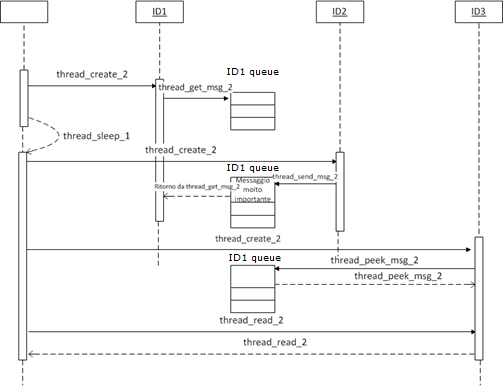
\includegraphics[width=12cm]{images/thread-example}
\caption{Execution flows in the third example.}
\label{fig:thread-example}
\end{figure}

\begin{verbatim}
start(X):- thread_create(ID1, thread1(ID1)),
           thread_sleep(200),
           thread_create(ID2, thread2(ID1)),
           thread_create(ID3, thread3(ID1,X)),
           thread_read(ID3, _),
           write('Father: done').

thread1(ID):- tell('threadLog.txt'),
              write('ID1: waiting for message'),
              thread_get_msg(ID, m(X)),
              write('ID1: message retrieved').

thread2(ID):- thread_send_msg( ID, m('critical message')),
              write('ID2: message sent').		

thread3(ID,X):- thread_peek_msg( ID, m(X)),
                write('ID3: trying to get message').
\end{verbatim}

More in detail, the father creates three threads identified by \texttt{ID1}, \texttt{ID2}, and \texttt{ID3}, which execute the goals \texttt{thread1/1}, \texttt{thread2/1}, and \texttt{thread3/2}, respectively: \texttt{ID1} is the message receiver/logger, \texttt{ID2} is the message sender, \texttt{ID3} is the task charged to monitor its brother's queue. To prevent races, the father waits for 200 ms after creating the first (message receiver) thread \texttt{ID1}, so that it is surely up and running when the message sender \texttt{ID2} and its brother \texttt{ID3} actually start.
Then, the father suspends its execution, waiting for \texttt{ID3} to terminate.

However, since \texttt{ID1} removes the message from its queue when reading (via \texttt{thread\_get\_msg/2}), \texttt{ID3} never finds anything when checking its brother's queue (via the non-blocking \texttt{thread\_peek\_msg/2} primitive): thus, its goal \texttt{thread3/2} always fails, causing the father's \texttt{thread\_read} to fail, too. As a result, the father's final write is never performed, either:

\begin{verbatim}
?- start(X).
no
\end{verbatim}
%
and the log file finally contains just

\begin{verbatim}
ID1: waiting for message
ID2: message sent
ID1: message retrieved
\end{verbatim}


%-------------------------------
\subsubsection{Synchronizing thread interactions}
%-------------------------------

In this producer/consumer example, the consumer's goal is to retrieve only the \textit{last} solution of the query \texttt{has\_child(bob,X)}, while the producer computes all the solutions to this query; the father coordinates the two tasks, by first creating the producer and the consumer, and then triggering the producer to generate all the possible solutions in sequence.

Without an explicit synchronisation mechanism, races would occur, causing the reader to read not \textit{the last} solution, but just ``one of'' the possible solutions, depending which thread is faster.

By suitably sequentialising the access to the producer's queue, the \texttt{mutex} semaphore guarantees that all solutions are produced \textit{before} the consumer can start reading, so that the last solution is actually read. (The execution flow diagram and the complete code are reported in Figure \ref{fig:thread-exampleMutex} on page \pageref{fig:thread-exampleMutex}.)

\begin{figure}
\centering
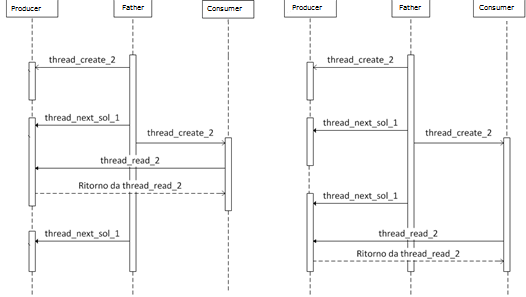
\includegraphics[width=13cm]{images/thread-exampleMutex}
\caption{Execution flows in the mutex example.}
%\label{fig:thread-exampleMutex}
%\end{figure}

\begin{Verbatim}[frame=single, samepage=true]
start:- thread_create(ID1, has_child(bob,X)),
        mutex_lock('mutex'),
        thread_create(ID2, read_child(ID1,X)),
        loop(1,5,1, ID1),
        mutex_unlock('mutex').

read_child(ID, X) :- mutex_lock('mutex'),
                     thread_read(ID, X),
                     mutex_unlock('mutex').

has_child(bob, alex).
has_child(bob, anna).
has_child(bob, mary).

loop(I, To, Inc, ThreadId) :- Inc >= 0, I > To, !. 
loop(I, To, Inc, ThreadId) :- Inc < 0, I < To, !. 
loop(I, To, Inc, ThreadId) :- thread_has_next(ThreadId), 
                              !, 
                              thread_next_sol(ThreadId), 
                              Next is I+Inc,
                              loop(Next, To, Inc, ThreadId).
loop(I, To, Inc, ThreadId).
\end{Verbatim}

\label{fig:thread-exampleMutex}
\end{figure}

The first child, \texttt{ID1}, is the solution finder \& producer: its task is to generate the solutions of the given goal \texttt{has\_child(bob,X)}. When started, it looks for the first solution: once found, it suspends waiting for possible future requests for alternative solutions. These will be actually asked shortly, since the father triggers \texttt{ID1} to find all the alternative solutions (via the \texttt{loop/4} predicate, which embeds a call to \texttt{thread\_next\_sol}) just after generating its second child, the solution reader thread \texttt{ID2}.
In fact, \texttt{ID2}'s task is to retrieve the computed solution from \texttt{ID1}'s private queue: but due to the \texttt{thread\_read} semantics, it actually reads \texttt{ID1}'s result only when \texttt{ID1} has terminated. This is why explicit synchronisation is needed: otherwise, the reader would read ``one of'' the solutions, non-deterministically, depending on which thread is faster (this can be easily checked by commenting out the \texttt{mutex\_lock}/\texttt{mutex\_unlock} statements).

With the explicit \texttt{mutex} semaphore, interactions are sequentialised: as long as the father holds the lock, the reader cannot retrieve any solution. Since the lock is released only after all the solutions have been explored, the reader will actually get only the last computed solution, \texttt{X / mary}.

%-------------------------------
\subsubsection{Flattening and manipulating lists}
%-------------------------------

Table \ref{tab:thread-exampleFlatList} on page \pageref{tab:thread-exampleFlatList} shows a sequential Prolog program that manipulates a list of (sub)lists. More precisely, it first flattens the list of lists into a single flat list, then sorts the obtained list and counts the occurrence of a given term in that list.

\begin{table}\small
\begin{Verbatim}[frame=single, samepage=true]
start(L, 0, T) :- !.
start([H|Tail], N, T) :-
    plain(H,L_plain),
    bubble(L_plain,L_ord),
    occurr_count(T,H,Count),
    C is N-1, start(Tail,C, T).

plain(L1,L2) :- plain(L1,[],L2).

plain([],ACC,ACC).
plain([H|REST],ACC,L2) :-
    H = [_|_],
    plain(H,ACC,ACC1),
    plain(REST,ACC1,L2).
plain([H|REST],ACC,L2) :-
    append(ACC,[H],ACC1),
    plain(REST,ACC1,L2).
plain(X,ACC,L2) :-
    append(ACC,[X],L2).

bubble(L1,L2) :- bubble(L1,0,L2).

bubble(L1,0,L2) :-
    sweep(L1,0,L2).
bubble(L1,0,L2) :-
    sweep(L1,1,LTMP),
    bubble(LTMP,0,L2).

sweep([X|[]],0,[X|[]]).
sweep([X,Y|REST1],CHANGED,[X|REST2]) :-
    X =< Y, sweep([Y|REST1],CHANGED,REST2).
sweep([X,Y|REST1],1,[Y|REST2]) :-
    X > Y, sweep([X|REST1],_,REST2).

occurr_count(T,L,N) :- occurr_count(T,L,0,N).

occurr_count(_,[],ACC,ACC).
occurr_count(T,[T|REST],ACC,N) :-
    ACC1 is ACC+1, occurr_count(T,REST,ACC1,N).
occurr_count(T,[_|REST],ACC,N) :- occurr_count(T,REST,ACC,N).
\end{Verbatim}
\caption{The sequential version of the list manipulation program.\\
         Query: \texttt{?- start([[[2,2],2,2,1],[4,[3],2],[9,8,9,2]], 3, 2).}}
\label{tab:thread-exampleFlatList}
\end{table}

To exploit concurrency, the program needs to be restructured, distributing the responsibilities among different threads.
As an example, we decided to delegate the list flattening and sorting to a child thread, maintaining the final occurrence counting on the main (father)'s thread: the result is shown in Table \ref{tab:thread-exampleFlatListConcurrent} on page \pageref{tab:thread-exampleFlatListConcurrent}, where the sequential and the concurrent versions are compared. The concurrent version showed a 16\% performance gain.

\begin{table}\small
\textit{Sequential version:}
\begin{Verbatim}[frame=single, samepage=true]
start(L, 0, T) :- !.
start([H|Tail], N, T) :-
    plain(H,L_plain),
    bubble(L_plain,L_ord),
    occurr_count(T,H,Count),
    C is N-1, start(Tail,C, T).
...
\end{Verbatim}

\textit{Concurrent version:}
\begin{Verbatim}[frame=single, samepage=true]
start(L, N, T) :-
    thread_create(ID, firstResp(L, N)),
    secondResp(L, N, T).

secondResp(L, 0, T):- !.
secondResp([H|Tail], N, T) :-
    occurr_count(T,H,Count),
    C is N-1, secondResp(Tail,C, T).

firstResp(L, 0) :- !.
firstResp([H|Tail], N) :-
    plain(H,L_plain),
    bubble(L_plain,L_ord),
    C is N-1, firstResp(Tail,C).
...
\end{Verbatim}
\caption{The sequential version (top) and the concurrent (bottom) version of the list manipulation program.\\
         Query: \texttt{?- start([[[2,2],2,2,1],[4,[3],2],[9,8,9,2]], 3, 2).}}
\label{tab:thread-exampleFlatListConcurrent}
\end{table}




%---------------------------------------------------------------------
\section{DCGLibrary}
\label{sec:dgc-library}
%---------------------------------------------------------------------

\noindent \emph{Library Dependencies}: BasicLibrary.

This library provides support for Definite Clause Grammars (DCGs) \cite{bra00}, an extension of context free grammars that have proven useful for describing natural and formal languages, and that may be conveniently expressed and executed in Prolog.
%
Note that this library is not loaded by default when a \tuprolog{} engine is created: it must be explicitly loaded by the user, or via a \texttt{load\_library} directive inside any theory using DCGs.

A DCG rule has the general form \verb|Head --> Body|: to distinguish terminal from nonterminal symbols, a phrase (that is, a sequence of terminal symbols) must be written as a Prolog list, with the empty sequence written as the empty list \verb|[]|.
%
The body can contain also executable blocks in parentheses, which are interpreted as normal Prolog rules.

Here is a simple example (see also Figure \ref{fig:dcg-example} on page \pageref{fig:dcg-example}):
%
\begin{verbatim}
    sentence --> noun_phrase, verb_phrase.
    verb_phrase --> verb, noun_phrase.
    noun_phrase --> [charles].
    noun_phrase --> [linda].
    verb --> [loves].
\end{verbatim}
%
To verify whether a phrase is correct according to the given grammar, the \texttt{phrase/2} or \texttt{phrase/3} predicates are used---the latter form providing an extra argument for the `remainder' of the input string not recognised as being part of the phrase.
%
Some examples follow:\\

\verb|?- phrase(sentence, [charles, loves, linda])|

\texttt{\textit{yes}}\\

\verb|?- phrase(sentence, [Who, loves, linda])|

\texttt{\textit{Who/charles}}

\texttt{\textit{Who/linda}}\\

\verb|?- phrase(sentence, [charles, loves, linda, but, hates, laura], R)|

\texttt{\textit{R/[but, hates, laura]}}\\

\begin{figure}
\centering
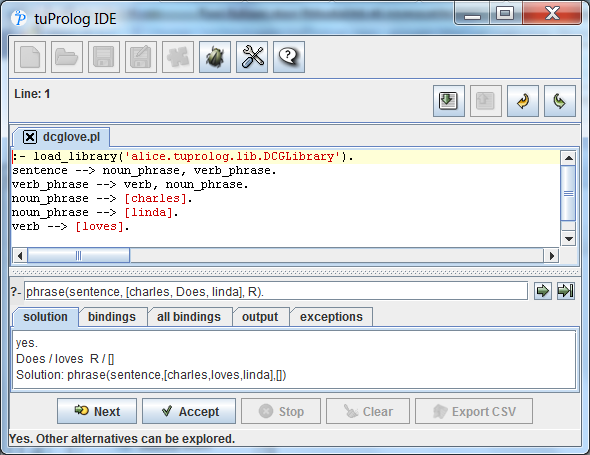
\includegraphics[width=7cm]{images/dcg-example}
\caption{The DCG Library example in the \tuprolog{} GUI (note the explicit library loading directive).}
\label{fig:dcg-example}
\end{figure}

%---------------------------------------------------------------------
\subsection{Predicates}
%---------------------------------------------------------------------

\noindent The classic built-in predicates provided for parsing DCG
sentences are:

\begin{itemize}
%
\item \bti{phrase/2}\\
    \noindent\bt{phrase(Category, List)} is true iff the list \bt{List} can be parsed as a phrase (i.e. sequence of terminals) of type \bt{Category}.
    \bt{Category} can be any term which would be accepted as a nonterminal of the grammar (or in general, it can be any grammar rule body), and must be instantiated to a non-variable term at the time of the call.
    This predicate is the usual way to commence execution of grammar rules.
    If \bt{List} is bound to a list of terminals by the time of the call, the goal corresponds to parsing \bt{List} as a phrase of type \bt{Category}; otherwise if \bt{List} is unbound, then the grammar is being used for generation.

    \template{phrase(+term, ?list)}

    \exception{error(instantiation\_error, instantiation\_error(\\
    Goal, ArgNo))} if \texttt{Category} is a variable. \texttt{Goal} is the goal where the problem occurred, \texttt{ArgNo} indicates the argument that caused the problem (obviously, \texttt{1}).

\item \bti{phrase/3}\\
    \noindent\bt{phrase(Category, List, Rest)} is true iff the segment between the start of list \bt{List} and the start of list \bt{Rest} can be parsed as a phrase (i.e. sequence of terminals) of type \bt{Category}.
    In other words, if the search for phrase Phrase is started at the beginning of list \bt{List}, then \bt{Rest} is what remains unparsed after \bt{Category} has been found.
    Again, \bt{Category} can be any term which would be accepted as a nonterminal of the grammar (or in general, any grammar rule body), and must be instantiated to a non variable term at the time of the call.

    \template{phrase(+term, ?list, ?rest)}

    \exception{error(instantiation\_error, instantiation\_error(\\
    Goal, ArgNo))} if \texttt{Category} is a variable. \texttt{Goal} is the goal where the problem occurred, \texttt{ArgNo} indicates the argument that caused the problem (obviously, \texttt{1}).

\end{itemize}

%---------------------------------------------------------------------
\subsection{Operators}
%---------------------------------------------------------------------

The full list of DCGLibrary operators, with their priority and associativity, is reported in Table \ref{tab:dcglibrary-operators}.

\begin{table}[h]
    \begin{center}{\small\tt
    \begin{tabular}{p{2cm}|p{3cm}|p{3cm}}\hline\hline
    Operator & Associativity & Priority \\ \hline
    --> & xfx & 1200\\
    \hline\hline
    \end{tabular}
    }\end{center}
    \caption{DCGLibrary operators.}\label{tab:dcglibrary-operators}
\end{table}


%---------------------------------------------------------------------
\section{ISOIOLibrary}
\label{sec:isoio-library}
%---------------------------------------------------------------------

The ISO specification requires a lot of I/O predicates---many more than \tuprolog{} IOLibrary supports.
%
Table \ref{fig:isoiolibrary-table} summarises the differences between \tuprolog{} IOLibrary and the ISO specifications.
%
\begin{figure}
  \centering
  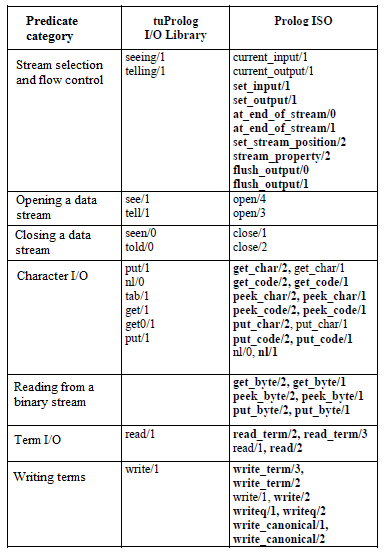
\includegraphics[width=10cm]{images/isoiolibrary-table}
  \caption{Comparison between the I/O predicates provided by IOLibrary and the ISO standard specification. Bold style indicates missing predicates, plain style indicates existing functionalities to be refactored, improved, or be provided with a different signature to be ISO-compliant.}\label{fig:isoiolibrary-table}
\end{figure}
%
The main reason for such a large number of differences is that the ISO Prolog standard defines very general concepts for I/O handling, aimed at supporting a wide variety of I/O modes and devices. More precisely:
\begin{itemize}
  \item \textbf{Sources} represent the resources from which data are read;
  \item \textbf{Sinks} represent the resources to which data are written.
\end{itemize}
%
Sources and sinks can be file, standard input/output stream, or any other resource supported by the underlying system: the only assumption is that each resource is associated to a sequence of bytes or characters.

\textit{Stream terms} provide a logical view of sources and sinks, and are used to identify a stream in I/O predicates. A stream term is a term respecting the following constraints:
\begin{itemize}
  \item it is a ground term;
  \item it is not an atom (this requirement means to distinguish stream terms from stream aliases--see below for details);
  \item it is not used to identify other streams at the same time.
\end{itemize}
%
The ISO standard does not specify whether the stream terms must result from an explicit source/sink opening by the \texttt{open/4} predicate, nor whether different sources/sinks must be represented by different stream terms at subsequent times: these issues are left to the specific implementation.

Moreover, each stream can be associated to a \textit{stream alias}---an atom used to refer to the stream. The association between a stream and its alias is created when the stream is opened, and automatically canceled when the stream is closed.
The same stream can be associated to multiple aliases simultaneously.
%
Two pre-defined streams exist that are always automatically open: the standard input (alias \texttt{user\_input}) and the standard output
(alias \texttt{user\_output}). Such streams must never be closed.

The ISO standard also introduces the concepts of \textit{current input stream} and \textit{current output stream}: initially, they default to the standard input and standard output above, but can be reassigned at any time via the \texttt{set\_input/1} e and \texttt{set\_output/1} predicates.
However, when such an input/output stream is closed, the current input/output stream must be re-set to its default value (i.e., the standard input/output, respectively).

One further concept is the \textit{stream position}, which defines the point where the next input/output will take place; syntactically, it is an implementation-dependent ground term.
The stream position is always supported, even by predicates whose operations do not change the position itself; to change the current position, the \texttt{set\_stream\_position/2} predicate is used.
When an output stream is repositioned, any output possibly present in the sink is overwritten; when an input stream is repositioned, instead, the content already available into the stream remains unaltered.

A stream that can be repositioned (that is, whose \texttt{reposition} property is true) must support also the \textit{end position} concept: the position of an input stream that has been completely read is represented by the \texttt{end-of-stream} atom, while any attempt to read beyond the end of stream causes the stream position to become \texttt{past-end-of-stream}.

On the other hand, output streams can be \textit{flushed} when necessary via the \texttt{flush\_output/1} predicate; a stream is automatically flushed before closing.


%---------------------------------------------------------------------
\subsection{Predicates}
%---------------------------------------------------------------------

\noindent ISOIOLibrary defines the following predicates:

\begin{itemize}

\item \bti{current\_input/1}\\
    \noindent\bt{current\_input} unifies the current input stream with the given argument.

    \template{current\_input(@Stream\_or\_alias)}

\item \bti{current\_output/1}\\
    \noindent\bt{current\_output} unifies the current output stream with the given argument.

    \template{current\_output(@Stream\_or\_alias)}


\item \bti{set\_input/1}\\
    \noindent\bt{set\_input} associates the current input to the provided argument, which can be either a stream\_term or an alias.

    \template{set\_input(@Stream\_or\_alias)}

    \exception{error(instantiation\_error, instantiation\_error)} if \textit{\texttt{Stream\_or\_alias}} is a variable.

    \exception{error(domain\_error, domain\_error(\texttt{stream\_or\_alias},\\
    \texttt{\textit{Stream\_or\_alias}}))} if \textit{\texttt{Stream\_or\_alias}} is neither a stream term nor a valid stream alias.

    \exception{error(existence\_error, existence\_error(\texttt{stream},\\
    \texttt{\textit{Stream\_or\_alias}}))} if \textit{\texttt{Stream\_or\_alias}} is not associated to an open stream.

    \exception{error(permission\_error, permission\_error(\texttt{input},\\
    \texttt{stream}, \texttt{\textit{Stream\_or\_alias}}))} if \textit{\texttt{Stream\_or\_alias}} is associated to an output stream.


\item \bti{set\_output/1}\\
    \noindent\bt{set\_output} associates the current output to the provided argument, which can be either a stream\_term or an alias.

    \template{set\_output(@Stream\_or\_alias)}

    \exception{error(instantiation\_error, instantiation\_error)} if \textit{\texttt{Stream\_or\_alias}} is a variable.

    \exception{error(domain\_error, domain\_error(\texttt{stream\_or\_alias},\\
    \texttt{\textit{Stream\_or\_alias}}))} if \textit{\texttt{Stream\_or\_alias}} is neither a stream term nor a valid stream alias.

    \exception{error(existence\_error, existence\_error(\texttt{stream},\\
    \texttt{\textit{Stream\_or\_alias}}))} if \textit{\texttt{Stream\_or\_alias}} is not associated to an open stream.

    \exception{error(permission\_error, permission\_error(\texttt{output},\\
    \texttt{stream}, \texttt{\textit{Stream\_or\_alias}}))} if \textit{\texttt{Stream\_or\_alias}} is associated to an input stream.

\item \bti{flush\_output/0} - \bti{flush\_output/1}\\
    \noindent\bt{flush\_output} flushes the output onto the stream associated to the provided argument, which can be either a stream\_term or an alias; if no argument is provided, the default output stream is flushed.

    \template{flush\_output(@Stream\_or\_alias)}\\
    \template{flush\_output}

    \exception{error(instantiation\_error, instantiation\_error)} if \textit{\texttt{Stream\_or\_alias}} is a variable.

    \exception{error(domain\_error, domain\_error(\texttt{stream\_or\_alias},\\
    \texttt{\textit{Stream\_or\_alias}}))} if \textit{\texttt{Stream\_or\_alias}} is not a valid stream term or alias.

    \exception{error(existence\_error, existence\_error(\texttt{stream},\\
    \texttt{\textit{Stream\_or\_alias}}))} if \textit{\texttt{Stream\_or\_alias}} is not associated to an open stream.

    \exception{error(permission\_error, permission\_error(\texttt{output},\\
    \texttt{stream}, \texttt{\textit{Stream\_or\_alias}}))} if \textit{\texttt{Stream\_or\_alias}} is associated to an input stream.


\item \bti{stream\_property/2}\\
    \noindent\bt{stream\_property} verifies whether the given stream has the given property, unifying \textit{\texttt{Property}} with the corresponding value.

    \template{stream\_property(?Stream, ?Property)}

    \exception{error(instantiation\_error, instantiation\_error)} if \textit{\texttt{Stream}} is a variable.

    \exception{error(domain\_error, domain\_error(\texttt{stream},\\
    \texttt{\textit{Stream}}))} if \textit{\texttt{Stream}} is not a stream term.

    \exception{error(domain\_error, domain\_error(\texttt{stream\_property},\\
    \texttt{\textit{Property}}))} if \textit{\texttt{Property}} is neither a variable nor a stream property.

    \exception{error(existence\_error, existence\_error(\texttt{stream},\\
    \texttt{\textit{Stream}}))} if \textit{\texttt{Stream}} is not associated to an open stream.


\item \bti{at\_end\_of\_stream/0} - \bti{at\_end\_of\_stream/1}\\
    \noindent\bt{at\_end\_of\_stream} succeeds if the \texttt{end\_of\_stream} property has either the \texttt{end\_of\_stream} or the \texttt{past\_end\_of\_stream} value. The zero-argument version checks the current input stream.

    \template{at\_end\_of\_stream(@Stream\_or\_alias)}\\
    \template{at\_end\_of\_stream}

    \exception{error(instantiation\_error, instantiation\_error)} if \textit{\texttt{Stream\_or\_alias}} is a variable.

    \exception{error(domain\_error, domain\_error(\texttt{stream},\\
    \texttt{\textit{Stream\_or\_alias}}))} if \textit{\texttt{Stream\_or\_alias}} is not a valid stream term or alias.

    \exception{error(existence\_error, existence\_error(\texttt{stream},\\
    \texttt{\textit{Stream\_or\_alias}}))} if \textit{\texttt{Stream\_or\_alias}} is not associated to an open stream.


\item \bti{set\_stream\_position/2}\\
    \noindent\bt{set\_stream\_position} is true if the stream position can be successfully set to the new \texttt{\textit{Position}} argument.

    \template{set\_stream\_position(@Stream\_or\_alias, @Position)}

    \exception{error(instantiation\_error, instantiation\_error)} if either \textit{\texttt{Stream\_or\_alias}} or \textit{\texttt{Position}} is a variable.

    \exception{error(domain\_error, domain\_error(\texttt{stream},\\
    \texttt{\textit{Stream\_or\_alias}}))} if \textit{\texttt{Stream\_or\_alias}} is not a valid stream term or alias.

    \exception{error(existence\_error, existence\_error(\texttt{stream},\\
    \texttt{\textit{Stream\_or\_alias}}))} if \textit{\texttt{Position}} is neither a valid stream position, nor a variable.

    \exception{error(permission\_error, permission\_error(\texttt{reposition},\\
    \texttt{stream}, \texttt{\textit{Stream\_or\_alias}}))} if the \texttt{reposition} property of this stream is false.


\item \bti{open/3} - \bti{open/4}\\
    \noindent\bt{open} succeeds if the stream can be opened according to the \texttt{mode} and \texttt{options} desired.

    \template{open(@Source\_Sink, @Mode, -Stream)}\\
    \template{open(@Source\_Sink, @Mode, -Stream, @Options)}

    \exception{error(instantiation\_error, instantiation\_error)} if either \textit{\texttt{Source\_sink}} or \textit{\texttt{Mode}} is a variable, or if \texttt{\textit{Options}} is a partial list or such a list contains a variable.

    \exception{error(type\_error, type\_error(atom, Mode))} if \textit{\texttt{Mode}} is a neither an atom nor a variable.

    \exception{error(type\_error, type\_error(list, Options))} if\\ \texttt{\textit{Options}} is neither a list nor a partial list.

    \exception{error(type\_error, type\_error(variable, Stream))} if \texttt{\textit{Stream}} is not a variable.

    \exception{error(domain\_error, domain\_error(\texttt{stream\_sink},\\
    \texttt{\textit{Source\_sink}}))} if \textit{\texttt{Source\_sink}} is not a valid stream source or sink.

    \exception{error(domain\_error, domain\_error(\texttt{io\_mode},\\
    \texttt{\textit{Mode}}))} if \textit{\texttt{Mode}} is an atom other than the prescribed \texttt{input} or \texttt{output}.

    \exception{error(domain\_error, domain\_error(\texttt{stream\_option},\\
    \texttt{\textit{Element}}))} if an \textit{\texttt{Element}} of the options list is neither a variable nor a valid stream option.

    \exception{error(existence\_error, existence\_error(\texttt{stream},\\
    \texttt{\textit{Source\_sink}}))} if the source /sink stream \textit{\texttt{Source\_sink}} does not exist.

    \exception{error(permission\_error, permission\_error(\texttt{open},\\
    \texttt{source\_sink}, \texttt{\textit{Source\_sink}}))} if the specified source/sink stream cannot be opened.

    \exception{error(permission\_error, permission\_error(\texttt{open},\\
    \texttt{source\_sink}, \texttt{alias(\textit{A})}))} if \texttt{alias(\textit{A})} is in the options list, and \texttt{\textit{A}} is already bound to another open stream.

    \exception{error(permission\_error, permission\_error(\texttt{open},\\
    \texttt{source\_sink}, \texttt{reposition(true)}))} if \texttt{reposition(true)} is in the options list, but the stream cannot be repositioned.


\item \bti{close/1} - \bti{close/2}\\
    \noindent\bt{close} closes the given stream, eliminating any associated alias(es).
    If the \texttt{force(true)} option is specified, the stream is immediately closed, ignoring any data not yet transferred (in the case of output streams); in any other case, the stream is flushed before closing. If the stream to be closed is the current stream, the latter will be associated to the standard input or output, as appropriate.

    \template{close(@Stream\_or\_alias)}\\
    \template{close(@Stream\_or\_alias, @Options)}

    \exception{error(instantiation\_error, instantiation\_error)} if either \textit{\texttt{Stream\_or\_alias}} is a variable, or \texttt{\textit{Options}} is a partial list or such a list contains a variable.

    \exception{error(type\_error, type\_error(list, Options))} if\\ \texttt{\textit{Options}} is neither a list nor a partial list.

    \exception{error(domain\_error, domain\_error(\texttt{stream\_or\_alias},\\
    \texttt{\textit{Stream\_or\_alias}}))} if \textit{\texttt{Stream\_or\_alias}} is not a valid stream term or alias.

    \exception{error(domain\_error, domain\_error(\texttt{close\_option},\\
    \texttt{\textit{Element}}))} if an \textit{\texttt{Element}} of the options list is neither a variable nor a valid close option.

    \exception{error(existence\_error, existence\_error(\texttt{stream},\\
    \texttt{\textit{Stream\_or\_alias}}))} if the stream \textit{\texttt{Stream\_or\_alias}} is not associated to an open stream.

    \exception{error(permission\_error, permission\_error(\texttt{open},\\
    \texttt{source\_sink}, \texttt{\textit{Source\_sink}}))} if the specified source/sink stream cannot be opened.

    \exception{error(permission\_error, permission\_error(\texttt{open},\\
    \texttt{source\_sink}, \texttt{alias(\textit{A})}))} if \texttt{alias(\textit{A})} is in the options list, and \texttt{\textit{A}} is already bound to another open stream.

    \exception{error(permission\_error, permission\_error(\texttt{open},\\
    \texttt{source\_sink}, \texttt{reposition(true)}))} if \texttt{reposition(true)} is in the options list, but the stream cannot be repositioned.


\item \bti{get\_char/2} - \bti{get\_char/1} - \bti{get\_code/2} - \bti{get\_code/1}\\
    \noindent\bt{get\_char} and \bt{get\_code} read the next char from the given stream, and unify it with the second argument---a character or an integer representing the character code, respectively; the single-argument version of these predicates read from the current input stream. Special cases are treated as follows:
    \begin{itemize}
      \item if the stream position is \texttt{past\_end\_of\_stream}, the action to be performed depends on the stream options specified when the stream was opened---namely, \texttt{eof\_action(\textit{Action})}(see above);
      \item if the stream position is \texttt{end\_of\_stream}, the EOF character is returned, and the stream position becomes \texttt{past\_end\_of\_stream}.
    \end{itemize}

    \template{get\_char(@Stream\_or\_alias, ?Character)}\\
    \template{get\_char(?Character)}\\
    \template{get\_code(@Stream\_or\_alias, ?Character\_code)}\\
    \template{get\_code(?Character\_code)}

    \exception{error(instantiation\_error, instantiation\_error)} if either \textit{\texttt{Stream\_or\_alias}} is a variable.

    \exception{error(type\_error, type\_error(in\_character, \textit{Character}))} if \texttt{\textit{Character}} is neither a variable nor a character.

    \exception{error(type\_error, type\_error(integer, \textit{Character\_code}))} if \texttt{\textit{Character\_code}} is neither a variable nor an integer.

    \exception{error(domain\_error, domain\_error(\texttt{stream\_or\_alias},\\
    \texttt{\textit{Stream\_or\_alias}}))} if \textit{\texttt{Stream\_or\_alias}} is not a valid stream term or alias.

    \exception{error(existence\_error, existence\_error(\texttt{stream},\\
    \texttt{\textit{Stream\_or\_alias}}))} if the stream \textit{\texttt{Stream\_or\_alias}} is not associated to an open stream.

    \exception{error(permission\_error, permission\_error(\texttt{input},\\
    \texttt{stream}, \texttt{\textit{Stream\_or\_alias}}))} if the stream in not an input stream.

    \exception{error(permission\_error, permission\_error(\texttt{input},\\
    \texttt{binary\_stream}, \texttt{\textit{Stream\_or\_alias}}))} if the stream in not a text stream.

    \exception{error(permission\_error, permission\_error(\texttt{input},\\
    \texttt{past\_end\_of\_stream}, \texttt{\textit{Stream\_or\_alias}}))} if the stream status is\\
    \texttt{end\_of\_stream(past)} and the option \texttt{eof\_action(true)} is active.

    \exception{error(representation\_error,  representation\_error(\texttt{\textit{\\
    Character}}))} if the entity read from the stream is not a character.

    \exception{error(representation\_error,  representation\_error(\texttt{\textit{\\
    Character\_code}}))} if the entity read from the input stream is an integer, but does not represent a character.


\item \bti{peek\_char/2} - \bti{peek\_char/1} - \bti{peek\_code/2} - \bti{peek\_code/1}\\
    \noindent\bt{peek\_char} and \bt{peek\_code} work identically to the \texttt{get\_char} and \texttt{get\_code} above, but leave the stream position unaltered after reading, so that a subsequent read operation returns the same character.

    \template{peek\_char(@Stream\_or\_alias, ?Character)}\\
    \template{peek\_char(?Character)}\\
    \template{peek\_code(@Stream\_or\_alias, ?Character\_code)}\\
    \template{peek\_code(?Character\_code)}

    \exception{}: the same as above.


\item \bti{put\_char/2} - \bti{put\_char/1} - \bti{put\_code/2} - \bti{put\_code/1}\\
    \noindent\bt{put\_char} and \bt{put\_code} are the writing counterparts of the \texttt{get\_char} and \texttt{get\_code} above; syntax and exceptions raised are basically identical, but the \texttt{Character} or \texttt{Character\_code} must be ground in this case---otherwise, an \texttt{instantiation\_error} occurs.

    \template{put\_char(@Stream\_or\_alias, +Character)}\\
    \template{put\_char(+Character)}\\
    \template{put\_code(@Stream\_or\_alias, +Character\_code)}\\
    \template{put\_code(+Character\_code)}

    \exception{}: the same as above, plus an \texttt{error(instantiation\_error, instantiation\_error)} if \texttt{Character} or \texttt{Character\_code} is a variable.

\item \bti{nl/0} - \bti{nl/1}\\
    \noindent\bt{nl} inserts a newline in the given stream.

    \template{nl(@Stream\_or\_alias)}\\
    \template{nl}

    \exception{error(instantiation\_error, instantiation\_error)} if either \textit{\texttt{Stream\_or\_alias}} is a variable.


\item \bti{read\_term/2} - \bti{read\_term/3} - \bti{read/1} - \bti{read/2}\\
    \noindent\bt{read\_term} succeeds if a term can be read from the given stream that can be unified with the \texttt{\textit{Term}} argument: \texttt{\textit{Options}} are considered only if the above unification succeeds. The \texttt{read} predicate works analogously, but no options can be specified. As usual, the no-stream versions (\bti{read\_term/2} and \bti{read/1}) operate on the current input stream.

    \template{read\_term(@Stream\_or\_alias, ?Term, +Options)}\\
    \template{read\_term(?Term, +Options)}\\
    \template{read(@Stream\_or\_alias, ?Term)}\\
    \template{read(?Term)}

    \exception{error(instantiation\_error, instantiation\_error)} if either \textit{\texttt{Stream\_or\_alias}} is a variable.

    \exception{error(instantiation\_error, instantiation\_error)} if \texttt{\textit{Options}} is either a partial list, or an element in the list is a variable.

    \exception{error(type\_error, type\_error(list, \textit{Options}))} if\\ \texttt{\textit{Options}} is neither a list nor a partial list.

    \exception{error(domain\_error, domain\_error(\texttt{stream\_or\_alias},\\
    \texttt{\textit{Stream\_or\_alias}}))} if \textit{\texttt{Stream\_or\_alias}} is not a valid stream term or alias.

    \exception{error(existence\_error, existence\_error(\texttt{stream},\\
    \texttt{\textit{Stream\_or\_alias}}))} if the stream \textit{\texttt{Stream\_or\_alias}} is not associated to an open stream.

    \exception{error(domain\_error, domain\_error(\texttt{read\_option},\\
    \texttt{\textit{Element}}))} if an element in the option list is neither a variable nor a valid read option.

    \exception{error(existence\_error, existence\_error(\texttt{stream},\\
    \texttt{\textit{Stream\_or\_alias}}))} if \textit{\texttt{Stream\_or\_alias}} is not associated to an open stream.

    \exception{error(permission\_error, permission\_error(\texttt{input},\\
    \texttt{stream}, \texttt{\textit{Stream\_or\_alias}}))} if the stream in not an input stream.

    \exception{error(permission\_error, permission\_error(\texttt{input},\\
    \texttt{binary\_stream}, \texttt{\textit{Stream\_or\_alias}}))} if the stream in not a text stream.

    \exception{error(permission\_error, permission\_error(\texttt{input},\\
    \texttt{past\_end\_of\_stream}, \texttt{\textit{Stream\_or\_alias}}))} if the stream status is\\
    \texttt{end\_of\_stream(past)} and the option \texttt{eof\_action(true)} is active.

    \exception{error(representation\_error,  representation\_error(\texttt{\textit{\\
    Flag}}))} if the entity read from the stream does not comply with the rules expressed by \texttt{\textit{Flag}}, which can be \texttt{max\_arity}, \texttt{max\_integer}, \texttt{min\_integer}.

    \exception{error(representation\_error,  representation\_error(\texttt{
    imp\_dep\_atom}))} if one or more characters in the input stream cannot form a valid token, or the character sequence cannot be transformed into a valid atom according to the current operator notation.

\item \bti{write\_term/2} - \bti{write\_term/3} - \bti{write/1} - \bti{write/2} - \bti{writeq/1} - \bti{writeq/2} - \bti{write\_canonical/1} - \bti{write\_canonical/2}\\
    These predicates are the writing counterparts of the \texttt{read\_term} and \texttt{read} predicates above: the given term is written on the given stream according to the specified write options, or following the default values\footnote{Namely: \texttt{quoted(false)}, \texttt{ignore\_ops(false)}, \texttt{numbervars(true)} for \texttt{write}, \texttt{quoted(true)}, \texttt{ignore\_ops(false)}, \texttt{numbervars(true)} for \texttt{writeq}, \texttt{quoted(true)}, \texttt{ignore\_ops(true)}, \texttt{numbervars(true)} for \texttt{write\_canonical}.} in the \texttt{write}, \texttt{writeq} and \texttt{write\_canonical} cases. Basically, the same considerations and exceptions above still apply.

    \template{write\_term(@Stream\_or\_alias, @Term, +Options)}\\
    \template{write\_term(@Term, +Options)}\\
    \template{write(@Stream\_or\_alias, @Term)}\\
    \template{write(@Term)}
    \template{writeq(@Stream\_or\_alias, @Term)}\\
    \template{writeq(@Term)}

    \exception{}: the same as above

%---------------------------------------------------------------------
%\subsubsection{Writing terms}
%---------------------------------------------------------------------

    When a term is written via \texttt{write\_term/3}, the following rules apply:

    \begin{itemize}
      \item if the term is a variable, a character is produced of the form \texttt{\_\textit{string}} where the string following the underscore are implementation-dependent. A variable occurring multiple times in the term is obviously converted into the same \texttt{\_\textit{string}} for each occurrence.
      \item if the term is an integer number, the corresponding string is produced; negative values starts with \texttt{-}.
      \item if the term is a real number, the corresponding string is produced; negative values starts with \texttt{-}. If the write option \texttt{quoted} is true, the produced string ensures that a subsequent \texttt{read\_term} can read it back correctly.
      \item if the term is an atom that could not be read back unless quoted, and the write option \texttt{quoted} is true, the produced string is quoted; otherwise it is not.
      \item if the term contains a main functor that \textit{is not} an operator, or the write option \texttt{ignore\_ops} is true, the term is written in the \textit{canonical form} (Table \ref{tab:isoiolibrary-write-terms}); otherwise it is not.
      \item if, instead, the term contains a main that \textit{is} an operator and the write option \texttt{ignore\_ops} is true, the term is written in the operator notation ((Table \ref{tab:isoiolibrary-write-terms}).
    \end{itemize}

    \begin{table}
      \footnotesize\centering
      \begin{tabular}{|p{6cm}|p{6cm}|}
        \hline
        \textit{Canonical form} & \textit{Operator notation}\\
        \hline
        For every term other than lists: & - The operator itself is returned either before
        (for prefix operators), or between (for infix operators) or after (for postfix operators) its arguments;\\
        - the main functor's atom; &  - a space is always inserted between the operator and its arguments;\\
        - the open parenthesis \texttt{'('}; & - for each argument, the same rules above are applied recursively; \\
        - each term argument, built applying the same rules recursively, in a comma-separated list; & - if one of the argument is also an operator, it is enclosed between parentheses. \\
        - the closed parenthesis \texttt{')'}; & \\
        \textbf{Example:} \texttt{2+3} becomes \texttt{+(2,3)} & \\
        \hline
        For lists (e.g. terms of the form \texttt{�.�(Head, Tail)}), the list notation is used if the write option \texttt{ignore\_ops} is false: & \\
        - an open square bracket \texttt{'['}; &  \\
        - the head argument, built applying the same rules recursively; & \\
        - the tail argument, built as follows; & \\
        \mbox{~~}- if the tail has the form \texttt{�.�(Head, Tail)}), a comma is produced and the above rule is triggered recursively; & \\
        \mbox{~~}- otherwise, if the tail is empty (e.g. \texttt{[]}), a close bracket is produced \texttt{']'} & \\
        \mbox{~~}- otherwise, a pipe symbol is produced \texttt{'|'} and these rules are re-applied recursively; at the end, a close bracket is produced \texttt{']'} & \\
        \hline
      \end{tabular}
      \caption{Term writing rules: canonical form and operator notation.}
      \label{tab:isoiolibrary-write-terms}
\end{table}


\item \bti{get\_byte/2} - \bti{get\_byte/1} - \bti{peek\_byte/2} - \bti{peek\_byte/1} - \bti{put\_byte/2} - \bti{put\_byte/1}\\
    \noindent\bt{get\_byte}, \bt{peek\_byte} and \bt{put\_byte} are the binary counterparts of the \texttt{get\_char}, \texttt{peek\_char} and \texttt{put\_char} above; syntax and exceptions raised are basically identical, with obvious changes (i.e., the wrong type of stream here is \texttt{text} instead of \texttt{binary}).

    \template{get\_byte(@Stream\_or\_alias, ?Byte)}\\
    \template{get\_byte(?Byte)}\\
    \template{peek\_byte(@Stream\_or\_alias, ?Byte)}\\
    \template{peek\_byte(?Byte)}\\
    \template{put\_byte(@Stream\_or\_alias, +Byte)}\\
    \template{put\_byte(+Byte)}

    \exception{}: see description above.

\end{itemize}





%---------------------------------------------------------------------
\subsection{Options}
%---------------------------------------------------------------------

The ISO standard defines options for stream creation, stream closure, and stream properties.

\noindent When a stream is opened via \texttt{open/4}:

\begin{itemize}
 \item \texttt{type(\textit{Type})} specifies the stream type---either a binary stream or a text stream (default);
 \item \texttt{reposition(\textit{Bool})} specifies whether the stream can be repositioned or not (see above);
 \item \texttt{alias(\textit{Alias})} defines \texttt{\textit{Alias}} as a stream alias for this stream;
 \item \texttt{eof\_action(\textit{Action})} specifies the value to be returned by a read predicate encountering the end-of-stream; possible values are \texttt{error}, to indicate that no further read is possible, or \texttt{eof\_code} \textit{(default)}, to indicate that the special \texttt{eof} value must be returned, or \texttt{reset}, meaning that the read position must be reset to the start of the stream. This is particulary useful on the console input.
\end{itemize}

\noindent Conversely, when a stream is closed via \texttt{close/1}-\texttt{/2}:

\begin{itemize}
 \item \texttt{force(\textit{Bool})} specifies whether the stream must be forcedly closed upon error: the default is \textit{false}. If the value is set to \textit{true}, the stream might remain in an inconsistent state, or data may be lost, when the forced closing occurs.
\end{itemize}

\noindent Stream properties are expressed via the \texttt{stream\_property(\textit{Stream}, \textit{Property})} predicate, where \texttt{\textit{Property}} is one of the following:

\begin{itemize}
 \item \texttt{file\_name(\textit{File})} if the stream is connected to a file, returns a unique identifier of the file;

  \item \texttt{mode(\textit{Mode})} is to be specified when the stream is opened: \texttt{\textit{Mode}} can be \texttt{read}, \texttt{write} or \texttt{append};

  \item \texttt{input} if the stream is connected to a source;

  \item \texttt{output} if the stream is connected to a sink;

  \item \texttt{alias(\textit{Alias})} returns the stream alias, if the stream has one;

  \item \texttt{position(\textit{Pos})} returns the current stream position, if the stream can be repositioned;

  \item \texttt{end\_of\_stream(\textit{End})} returns either \texttt{not}, if the stream is not at the end, or \texttt{at}, if the stream is precisely at the end, or \texttt{past} if the stream is past the end of the stream;

  \item \texttt{eof\_action(\textit{Action})} returns the \texttt{\textit{Action}} specified when the stream was opened, if there was one, or an implementation-dependent action associated to the stream, otherwise;

  \item \texttt{reposition(\textit{Bool})} returns whether the stream can be repositioned (\texttt{true} or \texttt{false});

  \item \texttt{type(\textit{Type})} returns whether the stream is a \texttt{binary} stream or a \texttt{text} stream.
\end{itemize}

\noindent The standard input and output streams are configured as in Table \ref{tab:isoiolibrary-user-streams}.

\begin{table}
  \centering
  \begin{tabular}{|p{5cm}|p{5cm}|}
    \hline
    \textbf{\texttt{user\_input}} & \textbf{\texttt{user\_output}}\\
    \hline
    \texttt{mode(read)} & \texttt{mode(append)} \\
    \texttt{input} & \texttt{output} \\
    \texttt{alias(user\_input)} & \texttt{alias(user\_output)}\\
    \texttt{eof\_action(reset)} & \texttt{eof\_action(reset)}\\
    \texttt{reposition(false)} & \texttt{reposition(false)}\\
    \texttt{type(text)} & \texttt{type(text)}\\
    \hline
  \end{tabular}
  \caption{The default configuration of the standard I/O streams.}
  \label{tab:isoiolibrary-user-streams}
\end{table}


\noindent Read properties can be specified in read predicates like \texttt{read\_term}, and can have the following forms:

\begin{itemize}
 \item \texttt{variables(\textit{Vars})}: when a term is read, \texttt{\textit{Vars}} is the list of variables found in the term; anonymous variables are included;

 \item \texttt{variable\_names(\textit{VNList})}: when a term is read, \texttt{\textit{VNList}} is unified with a list of \texttt{A=V} pairs, where \texttt{A} is an atom denoting a variable name in term read, and \texttt{V} is the corresponding variable in the term template; anonymous variables are not included in the list;

 \item \texttt{singletons(\textit{VNList})}: when a term is read, \texttt{\textit{VNList}} is unified with a list of \texttt{A=V} pairs, where \texttt{A} is an atom denoting a variable name in term read, and \texttt{V} is the corresponding variable in the term template; anonymous variables are not included in the list.
\end{itemize}

\noindent For instance, if a query like:

\texttt{?:- read\_term(st, T, [variables(VL),\\
\mbox{~~~~~~~~~~~~~~~~~~~~~~~~~}variable\_names(VN), singletons(VS)].}

\noindent reads a term such as \texttt{foo(A+Roger, A+\_)}, the result is:

\noindent
\texttt{T  / foo(Xl+X2, X1+X3)}\\
\texttt{VL / [Xl, X2, X3]}\\
\texttt{VN / ['A' = Xl, 'Roger' = X2]}\\
\texttt{VS / ['Roger' = X2]}

\noindent Basically, the term read is scanned for variables, which are named according to some implementation-dependent template (e.g. \texttt{X1}, \texttt{X2}, \texttt{X3}); these names are used in the lists above, either to list all the variables (including the anonymous ones---see \texttt{X3} in \texttt{VL}), or to list the correspondence between the actual variable names and such placeholders (\texttt{VN} and \texttt{VS}, the latter including singleton variables only).

Analogously, write properties can be specified in write predicates like \texttt{write\_term}, and can have the following forms:

\begin{itemize}
 \item \texttt{quoted(\textit{Bool})}: specifies whether each atom of functor is quoted (usually because it comes from a previous \texttt{read\_term});

 \item \texttt{ignore\_ops(\textit{Bool})}: if true, each compound term is returned in a function notation. Any other option is ignored.

 \item \texttt{numbervars(\textit{Bool})}: if true, the terms of the form \texttt{'\$VAR'(N)} are replaced by a system-generated variable name that uses the \textit{N}th capital letter\footnote{\texttt{A} is considered the 0th letter.} followed by a the \texttt{N}/26 integer.
     For instance, \texttt{'\$VAR'(51)} produces \texttt{Z1}, since the 51th letter of the alphabet (mod 26) is \texttt{Z}, and 51/26=1.
\end{itemize}


%---------------------------------------------------------------------
\section{SocketLibrary}
\label{sec:socket-library}
%---------------------------------------------------------------------

\noindent \emph{Library Dependencies}: BasicLibrary.

This library provides support for TCP and UDP sockets. To this end, the library provides functionalities for
\begin{itemize}
  \item handling server sockets---namely, creating and closing a server socket, and accepting incoming connections;
  \item handling client sockets---namely, opening a socket establishing a connection to a given address;
  \item handling client/server communication, both in synchronous and asynchronous mode.
\end{itemize}

As an example, let us first consider the following TCP server-side code:\\

\begin{verbatim}
server(X,Y,Z):- tcp_socket_server_open('127.0.0.1:4444', Sock,[]),
                tcp_socket_server_accept(Sock,ClientAddr,Slave),
                read_from_socket(Slave,X,[]),
                write_to_socket(Slave,echo(X)),
                read_from_socket(Slave,Y,[]),
                write_to_socket(Slave,echo(Y)),
                read_from_socket(Slave,Z,[]),
                write_to_socket(Slave,echo(Z)),
                tcp_socket_server_close(Sock).
\end{verbatim}

\noindent to be coupled with the following TCP client-side code:\\

\begin{verbatim}
client(X,Y,Z):- tcp_socket_client_open('127.0.0.1:4444',Sock),
                write_to_socket(Sock,test1),
                read_from_socket(Sock,X,[]),
                write_to_socket(Sock,test2),
                read_from_socket(Sock,Y,[]),
                write_to_socket(Sock,test3),
                read_from_socket(Sock,Z,[]).
\end{verbatim}

\noindent In this scenario, the client opens a connection towards the server -- that is supposed to be already up and running, waiting connection requests on its server socket  -- and starts exchanging messages with the server.


In the UDP case, the same example would become:\\

\begin{verbatim}
server(X):- udp_socket_open('127.0.0.1:4445',Sock2),
            udp_receive(Sock2, X , '127.0.0.1:4444',[]),
            udp_socket_close(Sock2).
\end{verbatim}

\noindent to be coupled with the following UDP client:\\

\begin{verbatim}
client(X):- udp_socket_open('127.0.0.1:4444',Sock),
            udp_send(Sock, test1,'127.0.0.1:4444'),
            udp_socket_close(Sock).
\end{verbatim}


%---------------------------------------------------------------------
\subsection{Predicates}
%---------------------------------------------------------------------

\noindent The following socket handling predicates are provided:

\begin{itemize}
%
\item \bti{tcp\_socket\_server\_open/3}\\
    \noindent\bt{tcp\_socket\_server\_open(+Address, -Socket, +Options)} is true iff \bt{Address} represents a valid Internet address, and \bt{Socket} can be unified with a newly-created server socket; \bt{Options} is a possibly-empty list of options---currently, only the maximum number od connection request can be specified in the form of the \texttt{backlog(\textit{N})} term: if unspecified, the default value is \texttt{backlog(0)}, meaning the queue is unlimited.

    \template{tcp\_socket\_server\_open(+term, -term, +list)}

    \exception{error(instantiation\_error, instantiation\_error(\\
    Goal, ArgNo))} if \texttt{Socket} is not a variable, or the address length is not equal to 5 during the transformation of \texttt{Address} from the \texttt{IP:Port} form to the byte array and port number inner form.

\item \bti{tcp\_socket\_server\_accept/3}\\
    \noindent\bt{tcp\_socket\_server\_accept(+ServerSocket, -ClientAddress,\\
    -ClientSlaveSocket)} is true iff \bt{ServerSocket} represents a valid server socket address, and \bt{ClientAddress} can be unified with the client address in the \texttt{\textit{Address}:\textit{Port}} form, and \bt{ClientSlaveSocket} can be unified with the newly-created client socket.

    \template{tcp\_socket\_server\_accept(+term, -term, -term)}

    \exception{error(instantiation\_error, instantiation\_error(\\
    Goal, ArgNo))} if \texttt{ServerSocket} is a variable, or is not bound to server socket.

\item \bti{tcp\_socket\_server\_close/1}\\
    \noindent\bt{tcp\_socket\_server\_close(+ServerSocket)} is true iff \bt{ServerSocket} represents a valid server socket; as a side effect, the socket is closed.

    \template{tcp\_socket\_server\_close(+term)}

    \exception{error(instantiation\_error, instantiation\_error(\\
    Goal, ArgNo))} if \texttt{ServerSocket} is a variable, or is not bound to server socket.

\item \bti{tcp\_socket\_client\_open/2}\\
    \noindent\bt{tcp\_socket\_client\_open(+Address, -Socket)} is true iff \bt{Address} represents a valid Internet address in the \texttt{\textit{Address}:\textit{Port}} form, a server is waiting for incoming connection at that address, and \texttt{Socket} is unified with a newly-created socket.

    \template{tcp\_socket\_client\_open(+term, -term)}

    \exception{error(instantiation\_error, instantiation\_error(\\
    Goal, ArgNo))} if \texttt{Socket} is not a variable, or the address length is not equal to 5 during the transformation of \texttt{Address} from the \texttt{IP:Port} form to the byte array and port number inner form.

\item \bti{write\_to\_socket/2}\\
    \noindent\bt{write\_to\_socket(+Socket, +Msg)} is true iff \bt{Socket} represents a valid socket with an open associated output stream, and \texttt{Msg} is a valid term representing the message to be sent; as a side effect, the message is sent onto the stream.

    \template{write\_to\_socket(+term, +term)}

    \exception{error(instantiation\_error, instantiation\_error(\\
    Goal, ArgNo))} if \texttt{Socket} is a variable, or is not bound to client socket, or \texttt{Msg} is a variable.

\item \bti{read\_from\_socket/2}\\
    \noindent\bt{read\_from\_socket(+Socket, -Msg, +Options)} is true iff \bt{Socket} represents a valid socket with an open associated input stream, and \texttt{Options} is a valid option list---currently, only a timeout in milliseconds can be specified; as a side effect, a message is read from the stream and unified with \texttt{Msg}. If no message is available, the primitive suspends until one arrives (synchronous behaviour).

    \template{read\_from\_socket(+term, -term, +list)}

    \exception{error(instantiation\_error, instantiation\_error(\\
    Goal, ArgNo))} if \texttt{Socket} is a variable, or is not bound to client socket, or \texttt{Msg} is a variable.

\item \bti{aread\_from\_socket/2}\\
    \noindent\bt{aread\_from\_socket(+Socket, +Options)} is the asynchronous version of the above primitive; again, it is true iff \bt{Socket} represents a valid socket with an open associated input stream, and \texttt{Options} is a valid option list. As a side effect, a message is eventually read from the stream and asserted into the current prolog theory via \texttt{asserta}.
    Two options are available: the first makes it possible to set a timeout in milliseconds, as above; the other makes it possible to specify that the message is eventually asserted at the end of the current theory (i.e. via \texttt{assertz}) instead of at the top (i.e. via \texttt{asserta}, the default behaviour).

    \template{aread\_from\_socket(+term, +list)}

    \exception{error(instantiation\_error, instantiation\_error(\\
    Goal, ArgNo))} if \texttt{Socket} is a variable, or is not bound to client socket (only client sockets can asynchronously read from a server).

\item \bti{udp\_socket\_open/2}\\
    \noindent\bt{udp\_socket\_open(+Address, -DatagramSocket)} is true iff \bt{Address} represents a valid Internet address in the \texttt{\textit{Address}:\textit{Port}} form, a server is waiting for incoming connection at that address, and \texttt{DatagramSocket} is unified with a newly-created datagram socket.

    \template{udp\_socket\_open(+term, -term)}

    \exception{error(instantiation\_error, instantiation\_error(\\
    Goal, ArgNo))} if \texttt{Socket} is not a variable, or the address length is not equal to 5 during the transformation of \texttt{Address} from the \texttt{IP:Port} form to the byte array and port number inner form.

\item \bti{udp\_socket\_close/1}\\
    \noindent\bt{udp\_socket\_close(DatagramSocket)} is true iff \bt{DatagramSocket} represents a valid datagram socket; as a side effect, the socket is closed.

    \template{udp\_socket\_close(+term)}

    \exception{error(instantiation\_error, instantiation\_error(\\
    Goal, ArgNo))} if \texttt{DatagramSocket} is a variable, or is not bound to datagram socket.

\item \bti{udp\_send/3}\\
    \noindent\bt{udp\_send(-DatagramSocket, +Msg, +AddressTo)} is true iff \texttt{Msg} is a valid term representing the message to be sent, and \texttt{AddressTo} represents the destination address in the \texttt{\textit{Address}:\textit{Port}} form; as a side effect, \bt{DatagramSocket} is bound to the datagram socket associated to the output stream, and the message is sent onto the stream.

    \template{udp\_send(+term, +term, +term)}

    \exception{error(instantiation\_error, instantiation\_error(\\
    Goal, ArgNo))} if \texttt{DatagramSocket} is a not variable, or the address length is not equal to 5 during the transformation of \texttt{AddressTo} from the \texttt{IP:Port} form to the byte array and port number inner form.

\item \bti{udp\_receive/4}\\
    \noindent\bt{udp\_receive(-DatagramSocket, -Msg, +AddressTo, +Options)} is true iff \\
    \texttt{AddressTo} represents the destination address in the \texttt{\textit{Address}:\textit{Port}} form, and \texttt{Options} is a possibly-empty option list; currently, the available options are \texttt{max\_msg\_size(+\textit{Size})}, whose default value is 4096 bytes, and \texttt{timeout(+\textit{Time})}, which specifies a timeout: a value of 0 stands for infinite waiting.
    Upon reception of a message, as a side effect, the \texttt{Msg} term is unified with the incoming message, and
    \bt{DatagramSocket} is bound to a datagram socket associated to the input stream.

    \template{udp\_receive(+term, +term, +term, +list)}

    \exception{error(instantiation\_error, instantiation\_error(\\
    Goal, ArgNo))} if \texttt{DatagramSocket} is not a variable, or the address length is not equal to 5 during the transformation of \texttt{AddressTo} from the \texttt{IP:Port} form to the byte array and port number inner form.

\end{itemize}

%---------------------------------------------------------------------
\subsection{Operators}
%---------------------------------------------------------------------

No operators are defined in this library.

%The full list of SocketLibrary operators, with their priority and associativity, is reported in Table \ref{tab:socketlibrary-operators}.
%
%\begin{table}[h]
%    \begin{center}{\small\tt
%    \begin{tabular}{p{2cm}|p{3cm}|p{3cm}}\hline\hline
%    Operator & Associativity & Priority \\ \hline
%%    --> & xfx & 1200\\
%    \hline\hline
%    \end{tabular}
%    }\end{center}
%    \caption{SocketLibrary operators.}\label{tab:socketlibrary-operators}
%\end{table}

%---------------------------------------------------------------------
\subsection{Use from the Java side: term hierarchy extension}
%---------------------------------------------------------------------

In order to support the use of sockets from the Java side, SocketLibrary enhances the Term hierarchy by
introducing four further \texttt{Term} types that represent sockets: more precisely, \texttt{AbstractSocket} (a direct child of \texttt{Term}) represents the generic socket, whose concrete realisations are provided by its three children--- \texttt{Client\_Socket} and \texttt{Server\_Socket} in the TCP case, \texttt{Dataggram\_Socket} in the UDP case.

Consequently, \texttt{AbstractSocket} redefines some \texttt{Term} methods and defines some new abstract methods, implemented in the derived classes \texttt{Client\_Socket} and \texttt{Server\_Socket}:
\begin{itemize}
  \item \texttt{public abstract boolean isClientSocket();}
  \item \texttt{public abstract boolean isServerSocket();}
  \item \texttt{public abstract boolean isDatagramSocket();}
  \item \texttt{public abstract Object getSocket();}
  \item \texttt{public abstract InetAddress getAddress();}
\end{itemize}

\noindent In order to show the use of the SocketLibrary functions from Java, here are some small code chunks used in the JUnit test suite:

{\footnotesize\begin{verbatim}
@Test
public void testTcp_socket_client_open_2() throws PrologException, PrologError {
    String theory="client(X) :- tcp_socket_client_open('127.0.0.1:4444',Sock).";
    engine2.setTheory(new Theory(theory));
    SolveInfo goal=engine2.solve("client(X).");
    assertTrue(goal.isSuccess());	
}

@Test
public void testTcp_socket_client_open_2() throws PrologException, PrologError {
    Struct Address=new Struct("127.0.0.1:4444");
    Term Socket= new Var();
    SocketLib lib= (SocketLib) engine2.getLibrary("alice.tuProlog.lib.SocketLib");
    boolean res=lib.tcp_socket_client_open_2(Address, Socket);
    assertTrue(res);
}

@Test
public void testWrite_to_socket_2() throws InvalidTheoryException,
                                           MalformedGoalException, PrologError {
    String theory = "client(X,Y,Z):tcp_socket_client_open('127.0.0.1:4444',Sock),"
                    + "write_to_socket(Sock,test1)."	
    engine2.setTheory(new Theory(theory));
    SolveInfo goal=engine2.solve("client(X,Y,Z).");
    assertTrue(goal.isSuccess());	
}
\end{verbatim}}
